\documentclass[12pt,letterpaper]{article}
\usepackage[margin=1in]{geometry}
\usepackage{fontspec,graphicx,booktabs,longtable,multirow,float,amsmath,amssymb}
\setmainfont{lmroman12-regular.otf}[BoldFont=lmroman12-bold.otf,ItalicFont=lmroman12-italic.otf]
\usepackage{natbib,setspace,verbatim}
\usepackage[normalem]{ulem}
\usepackage[font=small,labelfont=bf]{caption}
\usepackage[colorlinks=true,linkcolor=blue,citecolor=blue,urlcolor=blue]{hyperref}
\setcitestyle{round,semicolon,aysep={},yysep={;}}
\setlength{\parindent}{3em}
\setlength{\tabcolsep}{3pt}
\setlength{\emergencystretch}{2em}
\newcommand{\result}[1]{\ifcsname result:#1\endcsname\csname result:#1\endcsname\else\PackageError{replication}{Missing result #1}{}\fi}
\expandafter\def\csname result:accuracy.figure_2.carry_opponents.congeniality_no_incentive.estimate.one\endcsname{14.4}
\expandafter\def\csname result:accuracy.figure_2.carry_opponents.congeniality_incentive.estimate.one\endcsname{-3.4}
\expandafter\def\csname result:accuracy.figure_2.carry_opponents.interaction.estimate.one\endcsname{-17.9}
\expandafter\def\csname result:accuracy.figure_2.carry_opponents.interaction.p\endcsname{=0.055}
\expandafter\def\csname result:accuracy.figure_2.carry_opponents.interaction.ci\endcsname{[-36.12, 0.41]}
\expandafter\def\csname result:accuracy.figure_2.carry_opponents.incentive_uncongenial.estimate.one\endcsname{16.0}
\expandafter\def\csname result:accuracy.figure_2.carry_opponents.incentive_uncongenial.p\endcsname{=0.014}
\expandafter\def\csname result:accuracy.figure_2.carry_opponents.incentive_uncongenial.ci\endcsname{[3.32, 28.67]}
\expandafter\def\csname result:accuracy.figure_2.carry_supporters.congeniality_no_incentive.estimate.one\endcsname{12.0}
\expandafter\def\csname result:accuracy.figure_2.carry_supporters.congeniality_incentive.estimate.one\endcsname{13.9}
\expandafter\def\csname result:accuracy.figure_2.carry_supporters.interaction.estimate.one\endcsname{1.9}
\expandafter\def\csname result:accuracy.figure_2.carry_supporters.interaction.p\endcsname{=0.782}
\expandafter\def\csname result:accuracy.figure_2.carry_supporters.interaction.ci\endcsname{[-11.62, 15.44]}
\expandafter\def\csname result:accuracy.figure_3.carry_opponents.incentive_uncongenial.estimate.one\endcsname{6.9}
\expandafter\def\csname result:accuracy.figure_3.carry_opponents.incentive_uncongenial.p\endcsname{=0.120}
\expandafter\def\csname result:accuracy.figure_3.carry_opponents.incentive_uncongenial.ci\endcsname{[-1.81, 15.68]}
\expandafter\def\csname result:accuracy.figure_3.carry_supporters.incentive_uncongenial.estimate.one\endcsname{-0.3}
\expandafter\def\csname result:accuracy.figure_3.carry_supporters.incentive_uncongenial.ci\endcsname{[-7.66, 7.03]}
\expandafter\def\csname result:accuracy.figure_4.wage_opponents.congeniality_no_incentive.estimate.one\endcsname{27.3}
\expandafter\def\csname result:accuracy.figure_4.wage_opponents.congeniality_incentive.estimate.one\endcsname{16.3}
\expandafter\def\csname result:accuracy.figure_4.wage_opponents.interaction.estimate.one\endcsname{-11.0}
\expandafter\def\csname result:accuracy.figure_4.wage_opponents.interaction.p\endcsname{=0.138}
\expandafter\def\csname result:accuracy.figure_4.wage_opponents.interaction.ci\endcsname{[-25.54, 3.55]}
\expandafter\def\csname result:accuracy.figure_4.wage_opponents.incentive_uncongenial.estimate.one\endcsname{8.4}
\expandafter\def\csname result:accuracy.figure_4.wage_opponents.incentive_uncongenial.ci\endcsname{[-3.88, 20.60]}
\expandafter\def\csname result:accuracy.figure_4.wage_supporters.congeniality_no_incentive.estimate.one\endcsname{-10.7}
\expandafter\def\csname result:accuracy.figure_4.wage_supporters.congeniality_no_incentive.ci\endcsname{[-16.42, -5.06]}
\expandafter\def\csname result:accuracy.figure_si_4.conservative_republican.congeniality_no_incentive.estimate.one\endcsname{4.2}
\expandafter\def\csname result:accuracy.figure_si_4.conservative_republican.congeniality_incentive.estimate.one\endcsname{23.6}
\expandafter\def\csname result:accuracy.figure_si_4.conservative_republican.interaction.estimate.one\endcsname{19.5}
\expandafter\def\csname result:accuracy.figure_si_4.conservative_republican.interaction.ci\endcsname{[-8.49, 47.43]}
\expandafter\def\csname result:accuracy.figure_si_4.liberal_democrat.congeniality_no_incentive.estimate.one\endcsname{7.6}
\expandafter\def\csname result:accuracy.figure_si_4.liberal_democrat.congeniality_incentive.estimate.one\endcsname{-4.2}
\expandafter\def\csname result:accuracy.figure_si_4.liberal_democrat.interaction.estimate.one\endcsname{-11.8}
\expandafter\def\csname result:accuracy.figure_si_4.liberal_democrat.interaction.ci\endcsname{[-26.50, 2.90]}
\expandafter\def\csname result:accuracy.figure_si_5.carry_opponents.interaction.estimate.one\endcsname{-17.1}
\expandafter\def\csname result:accuracy.figure_si_5.carry_opponents.interaction.ci\endcsname{[-42.85, 8.72]}
\expandafter\def\csname result:accuracy.figure_si_6.carry_opponents.interaction.estimate.one\endcsname{-21.4}
\expandafter\def\csname result:accuracy.figure_si_6.carry_opponents.interaction.ci\endcsname{[-47.67, 4.90]}
\expandafter\def\csname result:accuracy.figure_si_8.wage_opponents.interaction.estimate.one\endcsname{-14.1}
\expandafter\def\csname result:accuracy.figure_si_8.wage_opponents.interaction.p\endcsname{=0.100}
\expandafter\def\csname result:accuracy.figure_si_8.wage_opponents.interaction.ci\endcsname{[-30.85, 2.73]}
\expandafter\def\csname result:cell.figure_2.carry_opponents.0.0.estimate.one\endcsname{41.0}
\expandafter\def\csname result:cell.figure_2.carry_opponents.1.0.estimate.one\endcsname{55.5}
\expandafter\def\csname result:cell.figure_2.carry_supporters.0.0.estimate.one\endcsname{42.6}
\expandafter\def\csname result:cell.figure_2.carry_supporters.1.0.estimate.one\endcsname{54.6}
\expandafter\def\csname result:cell.figure_3.carry_opponents.0.0.estimate.one\endcsname{25.6}
\expandafter\def\csname result:cell.figure_3.carry_opponents.0.1.estimate.one\endcsname{32.5}
\expandafter\def\csname result:cell.figure_3.carry_supporters.0.0.estimate.one\endcsname{33.6}
\expandafter\def\csname result:cell.figure_3.carry_supporters.0.1.estimate.one\endcsname{33.3}
\expandafter\def\csname result:cell.figure_4.wage_opponents.0.0.estimate.one\endcsname{62.0}
\expandafter\def\csname result:cell.figure_4.wage_opponents.1.0.estimate.one\endcsname{89.3}
\expandafter\def\csname result:rating.carry_opponents.interaction.estimate\endcsname{0.41}
\expandafter\def\csname result:rating.carry_opponents.interaction.p\endcsname{=0.336}
\expandafter\def\csname result:rating.carry_opponents.interaction.ci\endcsname{[-0.42, 1.23]}
\expandafter\def\csname result:rating.carry_supporters.interaction.estimate\endcsname{0.31}
\expandafter\def\csname result:rating.carry_supporters.interaction.p\endcsname{=0.344}
\expandafter\def\csname result:rating.carry_supporters.interaction.ci\endcsname{[-0.33, 0.95]}
\expandafter\def\csname result:rating.pooled.interaction.estimate\endcsname{0.34}
\expandafter\def\csname result:rating.pooled.interaction.p\endcsname{=0.180}
\expandafter\def\csname result:rating.pooled.interaction.ci\endcsname{[-0.16, 0.85]}
\expandafter\def\csname result:recall.recall_a.0.estimate.one\endcsname{213.9}
\expandafter\def\csname result:recall.recall_a.0.std_error.one\endcsname{5.5}
\expandafter\def\csname result:recall.recall_a.1.estimate.one\endcsname{212.5}
\expandafter\def\csname result:recall.recall_a.1.std_error.one\endcsname{4.9}
\expandafter\def\csname result:recall.recall_c.0.estimate.one\endcsname{103.1}
\expandafter\def\csname result:recall.recall_c.0.std_error.one\endcsname{2.7}
\expandafter\def\csname result:recall.recall_c.1.estimate.one\endcsname{105.2}
\expandafter\def\csname result:recall.recall_c.1.std_error.one\endcsname{4.7}
\expandafter\def\csname result:odds.study_2_high.carry_opponents.0.response_odds\endcsname{1.22}
\expandafter\def\csname result:odds.study_2_high.carry_opponents.1.response_odds\endcsname{0.84}
\expandafter\def\csname result:odds.study_2_low.carry_opponents.0.response_odds\endcsname{1.25}
\expandafter\def\csname result:odds.study_2_low.carry_opponents.1.response_odds\endcsname{1.06}
\expandafter\def\csname result:odds.study_3_high.carry_opponents.0.response_odds\endcsname{2.04}
\expandafter\def\csname result:odds.study_3_high.carry_opponents.1.response_odds\endcsname{1.68}
\expandafter\def\csname result:odds.study_3_low.carry_opponents.0.response_odds\endcsname{3.68}
\expandafter\def\csname result:odds.study_3_low.carry_opponents.1.response_odds\endcsname{2.41}
\expandafter\def\csname result:mean.1.gun_ban.estimate.one\endcsname{33.7}
\expandafter\def\csname result:mean.2.gun_ban.estimate.one\endcsname{35.7}
\expandafter\def\csname result:mean.2.wage_correct.estimate.one\endcsname{87.1}
\expandafter\def\csname result:mean.2.wage_support.estimate.one\endcsname{84.6}
\expandafter\def\csname result:mean.3.gun_ban.estimate.one\endcsname{39.5}
\expandafter\def\csname result:mean.3.wage_correct.estimate.one\endcsname{76.9}
\expandafter\def\csname result:mean.3.wage_support.estimate.one\endcsname{65.0}
\expandafter\def\csname result:welch.0.1.true.estimate\endcsname{1.05}
\expandafter\def\csname result:welch.1.1.true.estimate\endcsname{1.41}
\expandafter\def\csname result:model.gun_logit_position_1.classical.gun_congenial_gun_incentive.p\endcsname{=0.058}
\expandafter\def\csname result:worldview.liberal_democrat.discordant\endcsname{46.8}
\expandafter\def\csname result:worldview.conservative_republican.discordant\endcsname{14.6}
\expandafter\def\csname result:sample.1.n\endcsname{785}
\expandafter\def\csname result:sample.1.position\endcsname{686}
\expandafter\def\csname result:sample.2.n\endcsname{947}
\expandafter\def\csname result:sample.2.high\endcsname{692}
\expandafter\def\csname result:sample.2.high_pct\endcsname{73.1}
\expandafter\def\csname result:sample.2.wage_opponents\endcsname{129}
\expandafter\def\csname result:sample.3.n\endcsname{1062}
\expandafter\def\csname result:sample.3.high\endcsname{421}
\expandafter\def\csname result:sample.3.high_pct\endcsname{39.6}
\expandafter\def\csname result:sample.1.roster\endcsname{1207}
\expandafter\def\csname result:worldview.study_2.low.correlation\endcsname{0.16}
\expandafter\def\csname result:worldview.study_2.high.correlation\endcsname{0.41}
\expandafter\def\csname result:sample.1.workers\endcsname{749}
\expandafter\def\csname result:rating.alpha\endcsname{0.82}
\expandafter\def\csname result:confidence.gun.certain\endcsname{13.1}
\expandafter\def\csname result:confidence.gun.incorrect\endcsname{10.5}
\expandafter\def\csname result:confidence.wage.certain\endcsname{23.3}
\expandafter\def\csname result:confidence.wage.incorrect\endcsname{3.8}

\title{Motivated Responding in Studies of Factual Learning\thanks{We would like to thank Princeton Research in Experimental Social Science (PRESS) for financial support.
We are also very grateful to Dan Kahan for generously sharing experimental design details; Doug Ahler, Martin Bisgaard, Katie McCabe, Peter Mohanty, and Markus Prior for insightful comments on a previous draft; participants of the PRESS workshop for suggestions about the experimental design; and finally, the editor of this journal and three reviewers for their critical feedback and guidance.
The data and code necessary to replicate the results in this paper are available at \href{https://dataverse.harvard.edu/dataverse/polbehavior}{https://dataverse.harvard.edu/dataverse/polbehavior}.}}
\author{Kabir Khanna \and Gaurav Sood}
\date{}
% Original author text; only verified numerical, inferential, and exhibit corrections.
% Unchanged numeric literals describe design, stimuli, dates, citations, or externally reported benchmarks.
\begin{document}
\pagenumbering{roman}
\maketitle
\begin{center}\small Replication revision: reconstructed data and corrected exhibits.\end{center}
\thispagestyle{empty}



\begin{abstract}
\noindent Large partisan gaps in reports of factual beliefs have fueled concerns about citizens' competence and ability to hold representatives accountable. In three separate studies, we reconsider the evidence for one prominent explanation of these gaps---motivated learning. We extend a recent study on motivated learning that asks respondents to deduce the conclusion supported by numerical data. We offer a random set of respondents a small financial incentive to accurately report what they have learned. We find evidence consistent with a portion of what is taken as motivated learning being motivated responding. Incentives change reported answers, but do not separately identify truthful reporting, retrieval, and reasoning. Relatedly, recall estimates show no clear signed congeniality effect. However, the estimated increase in congeniality bias in judgments of credibility is positive but imprecise. In all, our findings suggest that motivated learning is less common than what the literature suggests, but do not establish that reduced bias in reporting is offset by increased bias in credibility judgments.
\end{abstract}

\newpage
\doublespacing
\pagenumbering{arabic}

Surveys of political knowledge frequently find large partisan differences in reported beliefs about policy-relevant facts. When Democrats control the White House, Democrats are likelier than Republicans to report that economic conditions are improving; the reverse holds true under a Republican administration \citep{bartels2002}. Similar patterns exist on answers to factual questions about healthcare \citep[e.g.,][]{nyhan2010}, foreign policy \citep[e.g.,][]{jacobson2010}, and social services \citep[e.g.,][]{jerit2012}, among other issues. In general, when people are surveyed about facts, they are more likely to report having beliefs that are {\it congenial} to their existing beliefs and attachments than beliefs that are {\it uncongenial}. While we expect values and preferences to differ in a pluralistic society, we do not expect disagreement over established facts. Factual disagreement fuels concerns about the public's ability to form preferences that are in line with their values or interests \citep[e.g.,][]{hochschild2001}, hold representatives accountable \citep[e.g.,][]{bartels2002}, and productively deliberate with each other \citep[][]{shapiro2008, muirhead2013}.

We consider two distinct explanations for differences in survey reports of factual beliefs: motivated learning and motivated responding.\footnote{Partisan gaps in factual beliefs may also arise from selective exposure to information (see \citealt{stroud2010}, though see also \citealt{prior2013}), and motivated assessments of credibility of information \citep[see, e.g.,][]{lord1979}.} According to the former, when people are presented with information, they are more likely to deduce that the information supports a congenial conclusion than an uncongenial conclusion \citep{jerit2012, kahan2013, kahan2017}. This bias in learning is thought to stem from the psychological drive to hold internally consistent beliefs that reflect positively on one's core attachments, such as political party, ideology, or cultural identity \citep{kunda1990}. Motivated learning is especially concerning from a normative standpoint. It suggests that even when people come across the same information, they can form very different beliefs about the conclusions supported by the information. (Note that learning about conclusions supported by information is different from believing that the conclusions are correct.) Such bias makes reducing gaps in factual beliefs yet harder---mere provision of accurate information is even less likely to work, and may even backfire \citep[see, e.g.,][]{nyhanreifler2010}.

However, differences in survey reports of factual beliefs do not always reflect differences in what people believe. Instead, they may be artifacts of the survey response process. Respondents sometimes give congenial but inaccurate answers in response to factual questions even when they have accurate but uncongenial facts at hand \citep{bullock2015, prior2015}. Other times, respondents are ignorant, having no relevant cognitions, and they offer a congenial answer as their best guess \citep{luskin2013}. In both cases, the survey response process inflates estimates of bias in factual beliefs. We extend this line of thinking to estimates of {\it learning}, the process that produces such beliefs. Like studies of stored cognitions, studies of learning may overstate bias if they do not account for motivated responding. 

We reassess the extent to which people learn in a motivated manner by simultaneously measuring motivated learning and motivated responding in three separate studies. Building on the design in \citet{kahan2017}---people are presented data from a social scientific study and asked to report the conclusion supported by the data---we incentivize a random set of respondents to honestly report the conclusion they actually think the data supports. Incentives reduce congeniality bias in reporting the study's result, suggesting that a portion of what appears to be motivated learning is in fact motivated responding. Correspondingly, we find no evidence that respondents selectively recall the data they were presented. However, point estimates of responsiveness to the incentive treatment differ by respondents' initial position on the issue under study. Moreover, the estimated increase in congeniality bias in study ratings is positive but imprecise. In all, our findings suggest that motivated learning is less common than what previous work suggests, but that motivated evaluation of information remains common.

\section*{Motivated Learning, Reporting, and Interpretation}

Psychological motivations are powerful in shaping how people process information. Broadly, people are motivated to both reach conclusions that are accurate and that are congenial to their beliefs \citep[see][]{kunda1990}. Most research in political psychology focuses on the latter, which \citeauthor{kunda1990} calls ``directional'' motivation. A great deal of research shows that directional motivations, like partisanship and ideology, bias evaluations of policy arguments \citep[e.g.,][]{lord1979, taber2006, bolsen2014} and of leaders \citep[e.g.,][]{bartels2002, lebo2007, kim2010}.

\subsection*{Motivated Learning}
While most research on motivated reasoning focuses on subjective attitudes, motivated reasoning may also influence factual learning. Suppose, for instance, that there exist some data that support an unequivocal conclusion relevant to public policy. And we ask an individual with an existing opinion on said policy to learn the conclusion supported by the data. The extent to which directional goals outweigh accuracy goals will be correlated with the probability the individual learns that the data support a conclusion that is congenial to them, even if this conclusion is incorrect. We refer to this phenomenon as {\it motivated learning}.

Motivated learning has received recent attention. For instance, \citet{nyhanreifler2010} find that partisans ignore correct information that contradicts their ideological worldview.\footnote{\citeauthor{nyhanreifler2010} test motivated learning using two-sided information flows. They instill false beliefs in respondents via misleading news stories and then attempt to reduce misperceptions with corrective stories. While this design lends external validity to their study, a one-sided context without contradictory information would afford a stricter test of motivated learning.} Similarly, \citet{jerit2012} find that partisans selectively learn party-relevant factual information. The authors present partisans with facts that reflect either positively or negatively on Democrats or Republicans. They find that partisans are more likely to learn congenial than uncongenial facts, e.g., Democrats are more likely to learn about the success of the Troubled Asset Relief Program than the size of the trade deficit. A major challenge in such experiments is cleanly manipulating information congeniality, while holding constant other attributes, such as topic and difficulty. We now consider a recent study that does just that.\footnote{
Many observational studies suggest motivated learning indirectly, by documenting partisan bias in factual beliefs \citep{bartels2002, shani2006, jerit2012}, though other observational studies find little partisan bias in factual beliefs \citep[e.g.,][]{gaines2007, blais2010}.}

\citet{kahan2017} cleverly repurpose a ``covariance detection task'' \citep[see][]{gilovich1991} to test whether people engage in motivated reasoning when processing policy-relevant data. Respondents see a $2 \times 2$ table with data on the relationship between banning concealed carry and rates of crime. The table's column headings are manipulated so that the data either support the conclusion that banning concealed reduces crime or the conclusion that banning concealed carry increases crime. When asked what result the data support, respondents are more likely to answer correctly when the data support a congenial claim than when the data support an uncongenial claim. That is, liberal Democrats are more likely to report the correct result when banning concealed carry reduces crime than when banning concealed carry increases crime, while the reverse is true among conservative Republicans. \citeauthor{kahan2017} use the terms {\it motivated numeracy} and {\it motivated cognition} to describe the phenomenon.

The finding is consistent with several other studies that show that people evaluate congenial and uncongenial claims differently, using different evidentiary standards and investing different amounts of effort in processing the information. When evaluating congenial claims, people tend not to be as thorough in searching for evidence \citep[e.g.,][]{kruglanksi1996, nickerson1998}, and evaluate available evidence more superficially and less skeptically \citep[e.g.,][]{chaiken1994}. On the other hand, when evaluating uncongenial claims, people are more skeptical and invest greater processing effort \citep[e.g.,][]{ditto1992, ditto1998, dawson2002}.  For instance, in the covariance detection task, respondents are more likely to only partially consider the data if doing so leads them to think that the data support a congenial conclusion \citep{dawson2002cella}. 

Building on this psychological literature, \citet{kahan2017} argue that our natural tendency to learn from data heuristically (i.e., using mental shortcuts) results in bias. For instance, when presented with tabular data, people tend to only consider the most salient datum in the table, for instance, the largest number, to deduce the conclusion supported by the data \citep[][p. 31]{gilovich1991}. If heuristic processing yields a congenial answer, people tend to stop processing, concluding that the data supports their beliefs. If heuristic processing instead yields an uncongenial result, people tend to look at the data more carefully to make sure they are correct. For instance, activating directional goals can motivate people to overcome the common error of neglecting `cell D' in a $2 \times 2$ table \citep{mata2015a, mata2015b}. This imbalance in scrutiny produces a {\it congeniality effect}: people learn congenial facts more readily than uncongenial facts. \citeauthor{kahan2017} argue that this effect increases with numeracy, because only respondents with sufficient numerical ability are capable of learning the correct result by considering all four cells.

Aside from asymmetric scrutiny, selective perception may also contribute to motivated learning. A long line of research suggests that expectation structures cognition \citep{hastorf1954, bechlivanidis2013, kahneman2013}. In our hurry to learn from data, for example, we misperceive data in ways that are consistent with our prior beliefs. For instance, when trying to distill information from a contingency table, people potentially misread the column or row labels in a way that suggests a congenial result. Alternatively, one might misread the numbers in the table. In all, either due to selective perception or an imbalance in scrutiny, people are thought to be more likely to learn correctly when the data are congenial than when they are uncongenial.

\subsection*{Motivated Responding}

Motivated responding concerns what survey respondents report on surveys, rather than what they have learned or know.\footnote{It is possible, even likely, that motivated responding also operates outside the survey context, explaining which beliefs people reveal in discussions with social networks, for example. However, in this paper, we focus on motivated responding in surveys.} In particular, it occurs when people with same underlying beliefs giving congenial answers more often than uncongenial answers when asked about their beliefs. In all, it contends that survey responses to factual questions reflect a mix of what people believe and what they wish to be true \citep{luskin2013, prior2015}.

People engage in motivated responding for a variety of reasons. Some deliberately misreport as a way to express their attitudes. For example, a survey respondent who vehemently opposes President Barack Obama may not admit knowing that the unemployment rate declined between 2008 and 2016 on a survey. The respondent may instead report a rise in unemployment to express their opposition. This kind of expressive self-presentation has been described as ``cheerleading'' \citep[e.g.,][]{gerber2009}. Others may misreport just to be consistent within a survey, ensuring that later answers do not contradict their earlier ones \citep[e.g.,][]{sears1983, lau1990, wilcox1993, palmer2001}. Yet others may engage in motivated responding to indicate their disbelief in information. For instance, in \citet{kahan2017}, a respondent may pick the congenial answer even after figuring out that the data support an uncongenial conclusion as a way to express their disbelief in the putative data.

In addition to actively misreporting what they believe, motivated responding may take more passive forms. For example, a respondent may withhold their beliefs by selecting ``Don't Know'' or skipping a question. Alternately, respondents who don't know the correct answer may report a congenial answer as their best guess. People may also engage in motivated responding without being consciously aware of it. For example, when asked a factual question in a survey, respondents may scan their memory for a longer time to come up with instances of congenial beliefs than uncongenial beliefs. In all, a variety of reasons exist why people may engage in motivated responding. Our study does not disentangle the various reasons behind motivated responding. Instead, our aim is to merely estimate the bias due to motivated responding in estimates of motivated learning derived from ordinary survey instruments.

While both motivated learning and responding fall under motivated reasoning, there are two major differences. First, motivating responding is about the survey response process, as opposed to learning. Motivated responding affects what people {\it say} they have learned, not what they actually learn. Second, and relatedly, we suspect that part of motivated responding is just ``cheap talk'' that people engage in to publicly protect their core attachments and beliefs. And to the extent that these public pronouncements are shallow, based not in what people deeply believe but what people are prepared to say publicly, these reported `beliefs' are unlikely to shape respondents' attitudes and behavior. On the other hand, uncongenial beliefs, which respondents are reluctant to express, may nonetheless influence attitudes and behavior. It is therefore important to distinguish between beliefs and instrumental or shallow responses.

A pair of recent studies find evidence that partisans engage in motivated responding on factual questions with political implications. \citet{bullock2015} and \citet{prior2015} find that partisans incorrectly report congenial beliefs, even when they know or could have inferred a more accurate answer. Both studies uncover motivated responding by boosting respondents' accuracy motivation. \citet{bullock2015} do so by offering respondents bonus payments for correct answers and for admitting their ignorance (by marking `don't know'), while \citet{prior2015} use a combination of bonus payments for correct answers, and textual appeals for responding honestly. Importantly, neither of the treatments provide any additional information. Therefore, any change in responses can be attributed to a change in respondents' motivation, rather than a change in their knowledge. Both studies find that, consistent with motivated responding, accuracy incentives substantially reduce partisan bias---by as much as half. 

Because studies of knowledge and learning rely on similar survey instruments, discovery of motivated responding on questions about stored knowledge suggests that estimates of motivated learning may also be inflated. To uncover motivated responding, we borrow a design feature of \citet{prior2008}, \citet{bullock2015}, and \citet{prior2015}, offering a random set of respondents small monetary incentives to accurately report their beliefs. To minimize the possibility that incentives affect processing of information, we present information about incentives \textit{after} respondents have seen the information and can no longer revisit it. These incentives increase respondents' motivation to honestly answer the which conclusion they think the data support. Respondents who would ordinarily offer a congenial answer as their best guess or as an act of political expression may be nudged to think more carefully or be more truthful. We therefore hypothesize that this treatment will attenuate the congeniality effect that \citet{kahan2017} and others observe.

More specifically, we hypothesize that incentives will increase the probability of answering correctly when the correct answer is uncongenial. If respondents learn the uncongenial result correctly, and then knowingly report an incorrect answer, incentives should encourage them to reveal their true belief. If respondents offer an incorrect, congenial response as their best guess, incentives should increase the probability that they will guess more evenhandedly. In both scenarios, incentives should increase correctness. However, we do not expect incentives to significantly increase correctness in the congenial condition, because here the congenial answer is the correct answer. We present our hypothesized pattern of results in a graphical format in Figure~\ref{fig:hypo}. The vertical axis represents the probability of answering correctly, and the dashed lines indicate the size of the congeniality effect. Incentives reduce the congeniality effect by increasing the probability of answering correctly in the uncongenial condition.

\begin{figure}[htbp]
  \centering
  \caption{Hypothesized Pattern of Results. Probability of correctly reporting study's result by experimental condition. Dashed vertical lines indicate congeniality effect, i.e., difference in probability of answering correctly between congenial and uncongenial conditions. We hypothesize that incentives will reduce the congeniality effect by increasing the probability of answering correctly in the uncongenial, but not the congenial, condition.}
\vspace{5mm}
   \includegraphics[page=7,width=.9\linewidth,trim=85 114 82 254,clip]{../data/reference/manuscript/Motivated Responding in Studies of Factual Learning.pdf}
\label{fig:hypo}
\end{figure}

\subsection*{Motivated Interpretation}
Directional motivations affect not just what people learn and report but also how credible people think a study is. Previous work suggests that people are more likely to question a study's credibility when its results are uncongenial than when they are congenial \citep[e.g.,][]{lord1979, kunda1990, ditto1992}. This phenomenon likely stems from the more general tendency to spend greater time and effort scrutinizing and refuting uncongenial claims than congenial claims, known as disconfirmation bias \citep[e.g.,][]{edwards1996, taber2006}. We therefore expect a congeniality effect on subjective study ratings: respondents will rate the same study as more convincing and well executed when its result is congenial than when it is not. And we expect this congeniality effect to be more pronounced when we incentivize respondents to report the correct study result, because respondents who admit an uncongenial result should be even more likely to report that the study behind the result is unconvincing.\footnote{We do not incentivize study ratings, because unlike the question about study's result, ratings are inherently subjective. Therefore, the logic of providing incentives to be accurate on subjective questions is unclear. Correspondingly, even if we were to provide incentives, we would not be able to interpret the results unambiguously.} 

\section*{Research Design}

To distinguish between motivated learning and motivated responding, we conduct three experiments that build upon the original design of \citet{kahan2017}. In particular, we add an orthogonal manipulation, offering participants a small monetary incentive to accurately report what they have learned. The $2 \times 2$ design enables us to test whether incentives reduce the congeniality effect, which has been interpreted as evidence for motivated learning. In addition to measuring the outcome used by \citeauthor{kahan2017}, we also measure subjective ratings of the study to examine whether the study's congeniality influences its perceived credibility. Below we elaborate on each of these extensions.

In Study 1, we asked respondents to read a summary of a hypothetical study on gun control. A preface to the study described its purpose: a city government is trying to decide whether or not to ban private citizens from carrying concealed weapons and wants to know if doing so would increase or decrease crime. After the preface, the study was briefly summarized: researchers compared changes in annual crime rates in cities that had banned concealed carry with changes in annual crime rates in cities that had not banned concealed carry. A $2 \times 2$ contingency table with the study's putative results came next.

Following \citet{kahan2017}, we manipulated the conclusion supported by the study by switching the column labels. In Table~\ref{tab:antigun}, cities that banned concealed carry were more likely to experience a crime {\it decrease} relative to cities that did not ban concealed carry. This result can be learned by comparing the ratios of cities in the first row (75:223 or about 1:3) and the second row (21:107 or about 1:5). Flipping the column labels produces the opposite result---the data now indicate that cities that banned concealed carry saw {\it increases} in crime (see Table~\ref{tab:progun} below).

\singlespacing
\begin{table}[h]
\centering
\caption {Oppose Concealed Carry} \label{tab:antigun}
\begin{tabular}{|l|l|l|}
\hline 
  & Increase in crime  & Decrease in crime \\\hline
  Cities that \underline{did} ban carrying     & \multirow{2}{*}{223 cities} & \multirow{2}{*}{75 cities} \\ 
  concealed handguns in public           &               & \\ \hline
  Cities that \underline{did not} ban carrying & \multirow{2}{*}{107 cities} & \multirow{2}{*}{21 cities} \\ 
  concealed handguns in public           &               &  \\\hline
\end{tabular}
\end{table}

\begin{table}[h]
\centering
\caption {Support Concealed Carry} \label{tab:progun}
\begin{tabular}{|l|l|l|}
\hline 
  & Decrease in crime & Increase in crime \\\hline
  Cities that \underline{did} ban carrying     & \multirow{2}{*}{223 cities} & \multirow{2}{*}{75 cities} \\ 
  concealed handguns in public           &               & \\ \hline
  Cities that \underline{did not} ban carrying & \multirow{2}{*}{107 cities} & \multirow{2}{*}{21 cities} \\ 
  concealed handguns in public           &               &  \\\hline
\end{tabular}
\end{table}
\doublespacing
\vspace{5mm}

After presenting the summary of the study, we asked respondents whether cities with a ban were more likely to experience an {\it increase} or {\it decrease} in crime than cities without a ban. This question serves as our primary dependent variable. Note that it is strictly factual in nature. It simply asks which of two descriptions is consistent with the data. The question does not ask the respondents to assess a causal claim, evaluate gun control, or indicate their faith in the study. Respondents could not access the study description and table when picking which of the conclusions were supported by the data. At the end of the survey, respondents were debriefed and informed that the data were not real.

To measure motivated responding, we independently manipulated respondents' motivation to give the answer they thought was correct. We offered a random set of respondents a small `nudge,' an additional \$0.10 for the correct answer.  Keeping the amount small has the virtue of not raising respondents' suspicions---some respondents may take a larger amount as cue that uncongenial answer is the right one. As to whether the small nudge is sufficient, we strictly cannot say, but note that \citet{prior2015} uncover about same amount of motivated responding by emphasizing the importance of accuracy without any extra money as they do by offering another \$1 for the correct answer. To ensure that incentives did not affect how respondents processed the contingency table in the treatment condition, we withheld any information about the incentive until after they had seen the table, and could no longer return to it. The control group was not offered incentives.

After measuring the primary dependent variable, we asked respondents to rate how convincing and how well done they found the concealed carry study. Each rating was measured on a 0-10 scale. We also asked respondents to recall the numbers in the contingency table at the end of the survey, in order to test whether respondents are more likely to remember congenial data than uncongenial data. To minimize respondent disengagement, we offered an additional \$0.05 for each number recalled correctly.

In Study 2, we readministered the concealed carry task and added another task following it. In the second task, respondents were presented with a study on the impact of raising the minimum wage. Again, respondents were asked to indicate its result based on tabular data. The minimum wage task was very similar to the concealed carry task in design, with two important differences (aside from the change in topic). First, with the intention of making it easier to learn the correct result, we replaced cell frequencies with percentages in the table. The percentage of correct responses was higher, although topic, format, and task order also differed, so this comparison does not identify the effect of making the task easier. Second, we manipulated the study's congeniality by switching the row labels instead of the column labels in the table (see Supporting Information (SI) Section~\ref{sec:qwording}). We believe this is a cleaner manipulation as it holds constant the increase-to-decrease ratio in each row, and simply changes the policy associated with each ratio. While lowering the task's difficulty might change the congeniality effect observed, we do not expect our changes to affect the degree of motivated responding. Lastly, randomization in the second task was conducted independently of the first, but the sequence of the two tasks was fixed.

In Study 3, we readministered both the concealed carry and minimum wage tasks on a more representative sample. Following our hypothesis that incentives influence responses in the uncongenial condition, we presented all respondents with an uncongenial version of the concealed carry task (based on their pre-treatment attitudes) and randomized incentives as in Studies 1 and 2. This simpler design allows us to conserve resources while testing our central theoretical claim that incentives increase correctness in the uncongenial condition. Additionally, we replicated the full $2 \times 2$ minimum wage task. The purpose of Study 3 was to gather confirmatory evidence and probe the generalizability of the estimates in Studies 1 and 2.

Before each relevant task, we measured attitudes toward banning concealed carry or raising the federal minimum wage to identify respondents who would find the result congenial or uncongenial. We expect respondents who oppose concealed carry to find a {\it decrease} in crime because of a concealed carry ban to be congenial, and an {\it increase} in crime uncongenial; we expect the opposite among respondents who support concealed carry. The same logic applies to the minimum wage task. We measured party identification, political ideology, and demographics prior to the experiments in each study. SI Section~\ref{sec:qwording} contains a complete description of the three studies and the complete wording of each task and question. In Studies 2 and 3, we omitted recall questions and ratings of the minimum wage study due to concerns about the length of the survey.

\section*{Data}

We recruited respondents from Amazon's Mechanical Turk (MTurk) in Studies 1 and 2.\footnote{MTurk is a micro-task market: workers complete small tasks, such as surveys, for money. For details of how samples are recruited on MTurk and general characteristics of the market, see \citet{buhrmester2011} and \citet{berinsky2012}.} We recruited `workers' for both studies by advertising a `task' of completing a short survey on `how people learn.' To assess whether our findings generalize beyond samples recruited on MTurk, we recruited respondents via Qualtrics in Study 3.
While it is not a ``gold standard,'' the Qualtrics sample is more representative of the general population, and respondents appear to be less attentive and detail-oriented than MTurk workers.
Study 1 was fielded in December 2013--January 2014, Study 2 in March 2015--April 2015, and Study 3 in August 2016.
For details of the recruited samples, see Table~\ref{tab:sample}.

While none of the samples are nationally `representative,' we can still learn a great deal from them. Multiple studies find that MTurk samples yield high-quality data and are more heterogeneous and representative than other common convenience samples, such as student samples \citep{buhrmester2011, berinsky2012, paolacci2014}. And recently, \citet{mullinix2015} replicate a broad array of experiments across different samples and find that treatment effects are broadly similar across samples. More generally, treatment effects vary across samples only when they are strongly conditioned by covariates that vary heavily across samples. We do not expect partisans on MTurk to differ from other partisans with respect to motivated reasoning. Multiple studies using MTurk samples find partisan bias in both stored knowledge \citep[e.g.,][]{chambers2014, ahler2015, chambers2015, bullock2015} and political judgments \citep[e.g.,][]{arceneaux2013, lyons2014, crawford2015a, crawford2015b, thibodeau2015}. In all, we think it likely that our treatment effects would be similar to studies using a nationally representative sample. 

Given the theoretical expectation that we should only observe motivated learning among respondents with sufficient numerical ability to complete the covariance detection task, we screened for high-numeracy respondents using a numeracy quiz in Study 1. The numeracy quiz was composed of the five easiest questions in \citet{weller2012} (see SI Section \ref{sec:numscreener} for exact items). We invited respondents answering four or more items correctly to participate in the full study. We use a threshold of four because \citet{kahan2017} find that the median respondent answers four items correctly on the full nine-item scale. In Studies 2 and 3, we invited all respondents to complete the main task, irrespective of numeracy, to ensure that our findings in Study 1 were not contingent on the relatively numerate MTurk sample.
In SI Section~\ref{sec:flow}, we report the source survey counts and overlapping analysis subsets by study.
Some characteristics are similar across numeracy groups, but Study 3 shows demographic differences (see Table~\ref{tab:sample} in SI Section~\ref{sec:sample}), but we also present their results separately in SI Section~\ref{sec:numeracy}.

In Study 1, the recruitment roster contains \result{sample.1.roster} records; \result{sample.1.n} records entered the full survey. Our main policy-congeniality analyses include \result{sample.1.position} records reporting a position on a concealed carry ban. The full Study 1 analysis sample represents \result{sample.1.workers} distinct workers. In Studies 2 and 3, the retained samples contain \result{sample.2.n} and \result{sample.3.n} records, respectively. Among those indicating a position, the percentages opposing concealed carry are \result{mean.1.gun_ban.estimate.one}\% in Study 1, \result{mean.2.gun_ban.estimate.one}\% in Study 2, and \result{mean.3.gun_ban.estimate.one}\% in Study 3. The percentages supporting a minimum-wage increase are \result{mean.2.wage_support.estimate.one}\% and \result{mean.3.wage_support.estimate.one}\% in Studies 2 and 3.\footnote{The original supplement reports national attitude benchmarks from a January 2013 CBS/New York Times survey and a January 2015 Associated Press/GfK poll. These external benchmarks are preserved in the original materials.}

The replication reconstructs the data from the original responses, corrects numeracy and party-leaning recodes, and calculates approximate age as interview year minus birth year. Study 2 rows are assumed to represent different workers. Analyses containing Study 1 records use worker-cluster CR2 uncertainty with contrast-specific degrees of freedom; other primary analyses use HC2. Tests are two-sided and intervals are 95\%. Historical coding and inference are retained separately. Clustering accounts for dependence between repeated records, but does not remove possible effects of repeated exposure to the task.

\section*{Results}

We begin by presenting results from the concealed carry task, first pooling data from Studies 1 and 2, followed by results from Study 3. We separate out Study 3 because the concealed carry task only included the uncongenial condition. We follow it with results from the minimum wage task, and end with describing impact of treatment on respondents' subjective study ratings.

If people learn in a motivated manner, the percentage of respondents answering correctly when the study's result is congenial should be greater than when the study's result is uncongenial. Respondents who {\it oppose} concealed carry should be more likely to answer correctly if the data support the conclusion that crime is more likely to decrease in cities with concealed carry bans than in cities without such bans. Among respondents who {\it support} concealed carry, the reverse should be true. We thus examine whether the congeniality manipulation increases the probability of answering correctly.\footnote{\citet{kahan2017} define congeniality on the basis of party identification and ideology. However, overlap between a composite of partisanship and ideology and attitude toward concealed carry is considerably short of 100\%. Across the three studies, \result{worldview.liberal_democrat.discordant}\% of self-described liberal Democrats oppose a ban on concealed carry, and \result{worldview.conservative_republican.discordant}\% of self-described conservative Republicans favor such a ban. We therefore opt for coding congeniality in terms of the attitude most directly related to the data being. Recoding congeniality on the basis of party identification and ideology, following \citeauthor{kahan2017}, changes the congeniality estimates (see SI Section~\ref{sec:kahan}).}

Before analyzing data from the covariance detection tasks, we compare partisanship, ideology, and demographics across experimental conditions (Table~\ref{tab:balance} in SI Section~\ref{sec:balance}). These balance checks do not independently establish successful randomization. We also assess associations between first-task treatments and second-task outcomes (Table~\ref{tab:spillover} in SI Section~\ref{sec:spillover}); nonsignificant coefficients do not establish the absence of spillover.
 
Figure~\ref{fig:pooled} plots the percentage answering correctly in the concealed carry task across Studies 1 and 2.\footnote{We subset high-numeracy respondents in Study 2 to ensure commensurability with Study 1. Study-specific results appear in Figures~\ref{fig:study1} and~\ref{fig:study2} in Section~\ref{sec:bystudy}.} Without incentives, concealed carry supporters answer correctly at rates of \result{cell.figure_2.carry_supporters.0.0.estimate.one}\% for an uncongenial result and \result{cell.figure_2.carry_supporters.1.0.estimate.one}\% for a congenial result. The congeniality effect is \result{accuracy.figure_2.carry_supporters.congeniality_no_incentive.estimate.one} percentage points. Among concealed carry opponents, the corresponding rates are \result{cell.figure_2.carry_opponents.0.0.estimate.one}\% and \result{cell.figure_2.carry_opponents.1.0.estimate.one}\%, a congeniality effect of \result{accuracy.figure_2.carry_opponents.congeniality_no_incentive.estimate.one} points. Both baseline differences exclude zero at the 95\% level.

\begin{figure}[p]
\centering
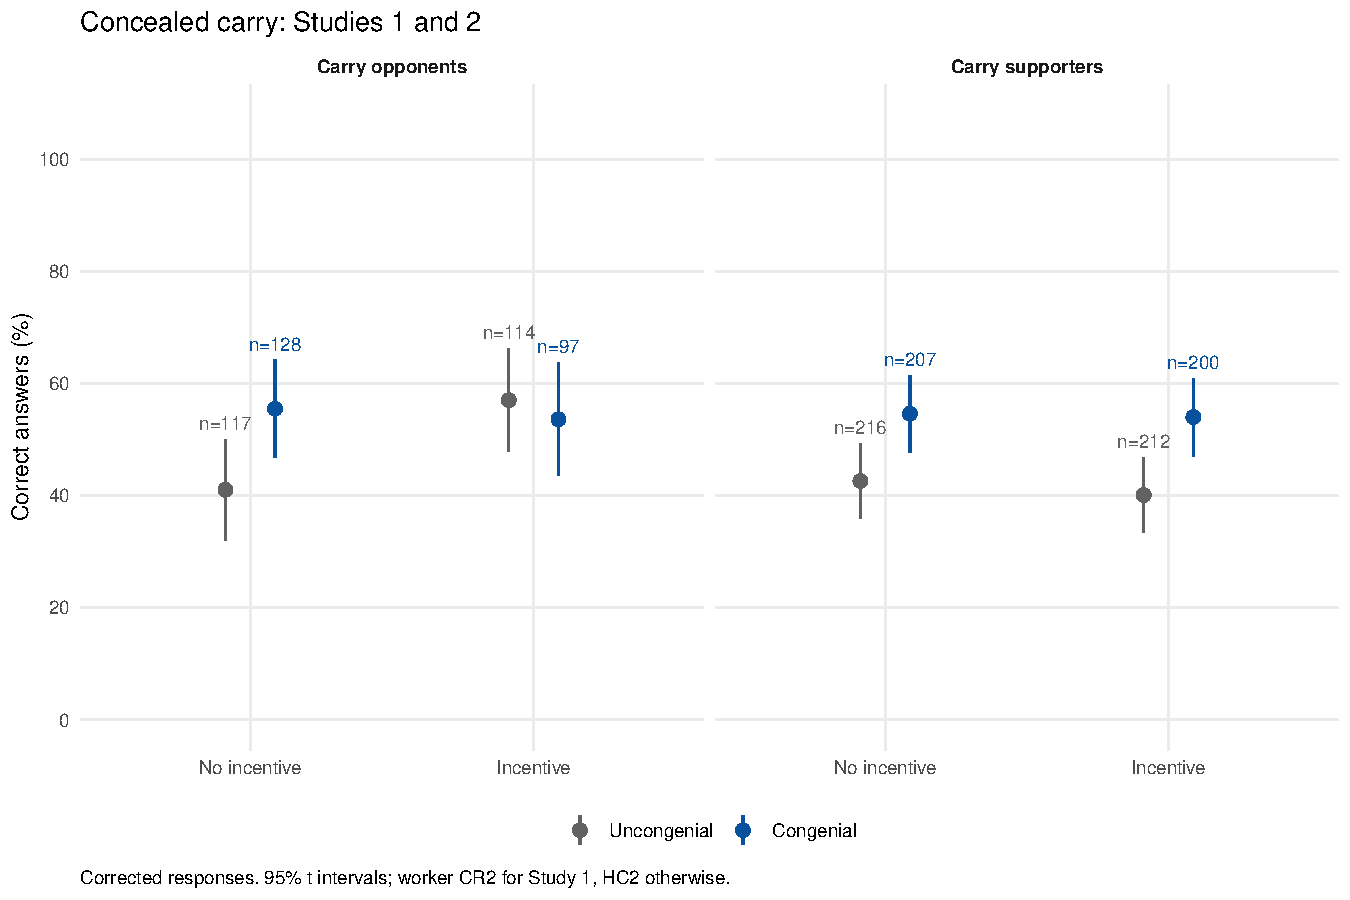
\includegraphics[width=.95\linewidth,height=.35\textheight,keepaspectratio]{../figs/figure_2.pdf}
\par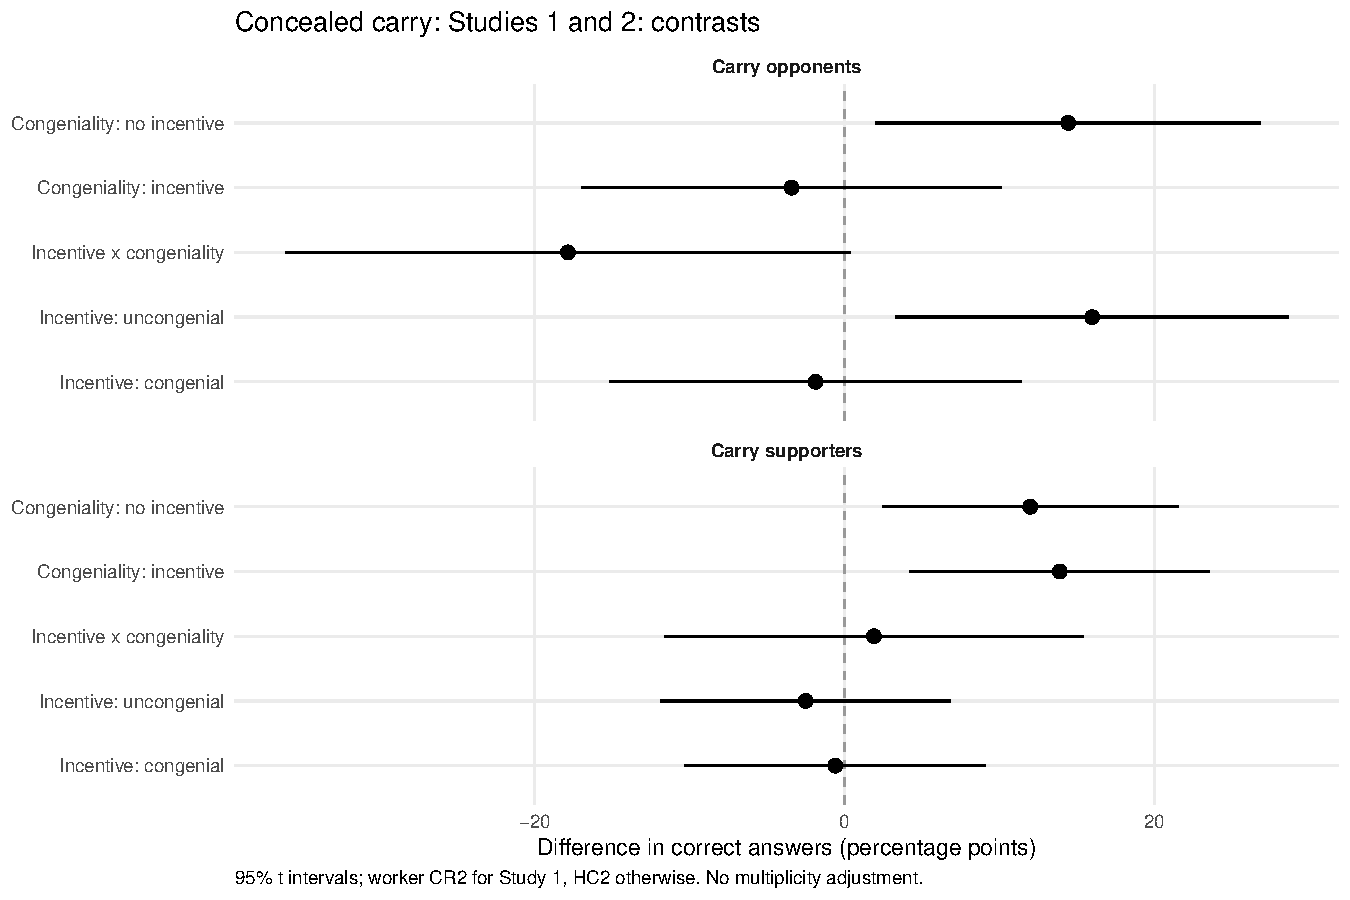
\includegraphics[width=.95\linewidth,height=.35\textheight,keepaspectratio]{../figs/figure_2_contrasts.pdf}
\caption{Concealed carry task, Studies 1 and 2. The upper plot shows correctness by condition; the lower plot shows contrasts. Groups are named in each panel. Study 2 is restricted to high numeracy. Intervals are 95\% worker-cluster CR2, treating Study 2 records as distinct workers.}\label{fig:pooled}
\end{figure}

We next examine the extent to which incentives reduce these congeniality effects, which \citet{kahan2017} and other scholars take as evidence of motivated learning. Incentives were revealed after respondents had seen the data and could not return to them. Recall estimates show no clear incentive effect (Tables~\ref{tab:recalla} and~\ref{tab:recallc} in SI Section~\ref{sec:recall}). These tests do not establish equivalence or rule out changes in retrieval or reasoning.

Among concealed carry supporters, the congeniality effect is \result{accuracy.figure_2.carry_supporters.congeniality_incentive.estimate.one} percentage points with incentives. Its change relative to the no-incentive condition is \result{accuracy.figure_2.carry_supporters.interaction.estimate.one} points (95\% CI \result{accuracy.figure_2.carry_supporters.interaction.ci}; $p\result{accuracy.figure_2.carry_supporters.interaction.p}$). We do not detect a reduction. A persistent congeniality gap is consistent with motivated learning, but does not identify it separately from remaining response bias.

Among concealed carry opponents, the point estimate of the congeniality effect falls from \result{accuracy.figure_2.carry_opponents.congeniality_no_incentive.estimate.one} to \result{accuracy.figure_2.carry_opponents.congeniality_incentive.estimate.one} percentage points. The difference-in-differences is \result{accuracy.figure_2.carry_opponents.interaction.estimate.one} points (95\% CI \result{accuracy.figure_2.carry_opponents.interaction.ci}; $p\result{accuracy.figure_2.carry_opponents.interaction.p}$). The interval includes zero. Consistent with our hypothesis, the point estimates attribute this reduction primarily to an increase in correctness in the uncongenial condition: \result{accuracy.figure_2.carry_opponents.incentive_uncongenial.estimate.one} points (95\% CI \result{accuracy.figure_2.carry_opponents.incentive_uncongenial.ci}; $p\result{accuracy.figure_2.carry_opponents.incentive_uncongenial.p}$).\footnote{Logistic specifications appear in Tables~\ref{tab:logit1} and~\ref{tab:logit2} in SI Section~\ref{sec:logit}.}

Study 3 included only the uncongenial version of the concealed carry task. Figure~\ref{fig:study3} displays correctness by policy position and incentive condition. Without incentives, \result{cell.figure_3.carry_supporters.0.0.estimate.one}\% of concealed carry supporters answer correctly, compared with \result{cell.figure_2.carry_supporters.0.0.estimate.one}\% in Studies 1 and 2. With incentives, Study 3 correctness is \result{cell.figure_3.carry_supporters.0.1.estimate.one}\%. The estimated incentive effect is \result{accuracy.figure_3.carry_supporters.incentive_uncongenial.estimate.one} points (95\% CI \result{accuracy.figure_3.carry_supporters.incentive_uncongenial.ci}).

Among Study 3 concealed carry opponents, correctness increases from \result{cell.figure_3.carry_opponents.0.0.estimate.one}\% without incentives to \result{cell.figure_3.carry_opponents.0.1.estimate.one}\% with incentives. The effect is \result{accuracy.figure_3.carry_opponents.incentive_uncongenial.estimate.one} percentage points (95\% CI \result{accuracy.figure_3.carry_opponents.incentive_uncongenial.ci}; two-sided $p\result{accuracy.figure_3.carry_opponents.incentive_uncongenial.p}$). The estimate is consistent in direction with Studies 1 and 2 but imprecise.

\begin{figure}[p]
\centering
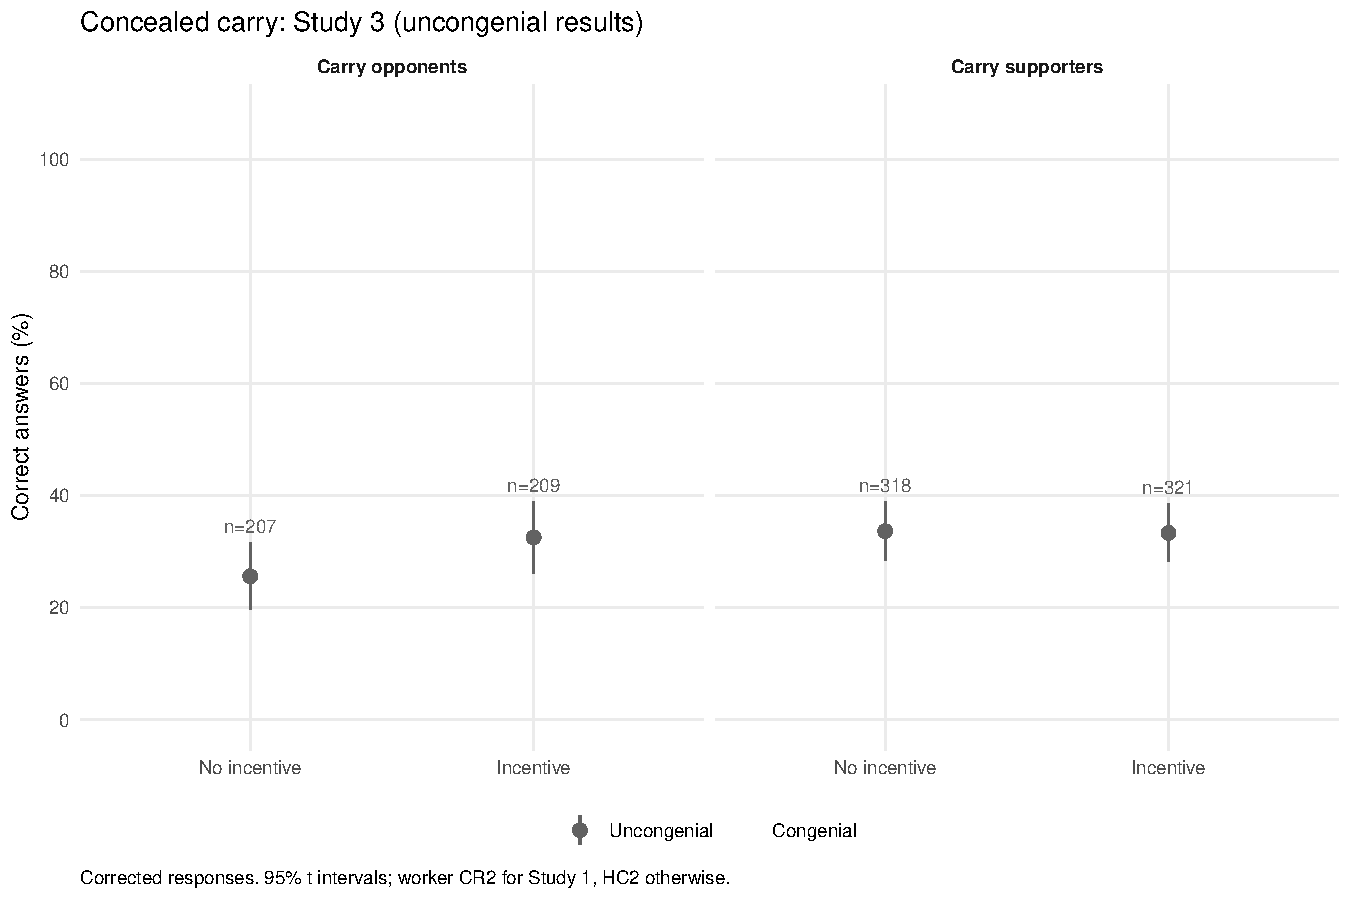
\includegraphics[width=.95\linewidth,height=.35\textheight,keepaspectratio]{../figs/figure_3.pdf}
\caption{Concealed carry task, Study 3. All stimuli are uncongenial. Points show correctness by incentive condition and policy position; intervals are 95\% HC2/t.}\label{fig:study3}
\end{figure}

We now turn to the minimum wage task in Studies 2 and 3. Overall correctness is \result{mean.2.wage_correct.estimate.one}\% in Study 2 and \result{mean.3.wage_correct.estimate.one}\% in Study 3. These rates are higher than in the concealed carry task, but differences in topic, format, and task order prevent attributing the difference solely to difficulty. Figure~\ref{fig:mwpool} pools Studies 2 and 3.\footnote{Study 2 includes \result{sample.2.wage_opponents} respondents opposing a minimum-wage increase. Study-specific results appear in Figures~\ref{fig:study2_wage} and~\ref{fig:study3_wage} in SI~\ref{sec:bystudy}.}

\begin{figure}[p]
\centering
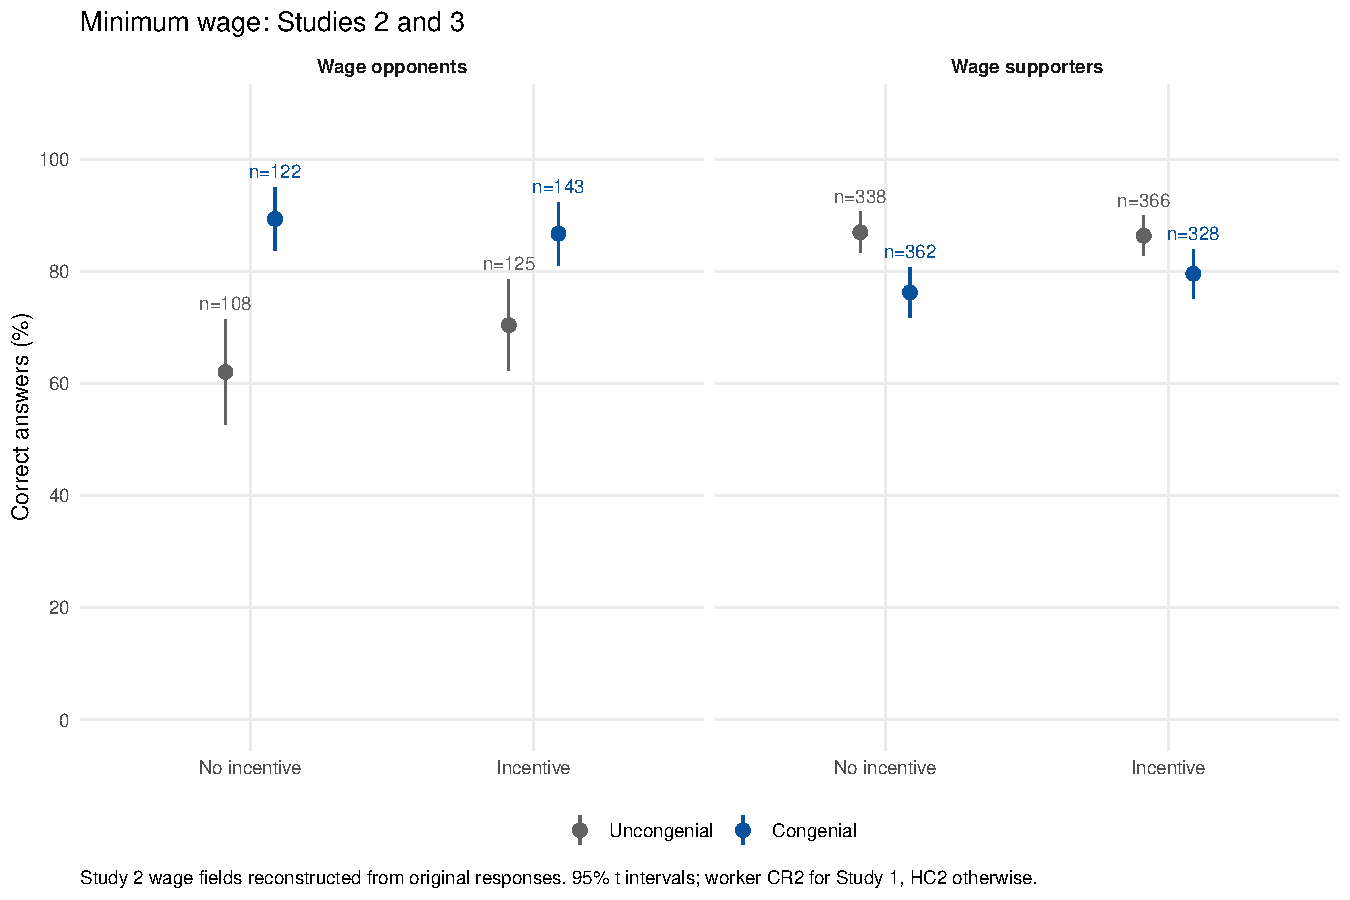
\includegraphics[width=.95\linewidth,height=.35\textheight,keepaspectratio]{../figs/figure_4.pdf}
\par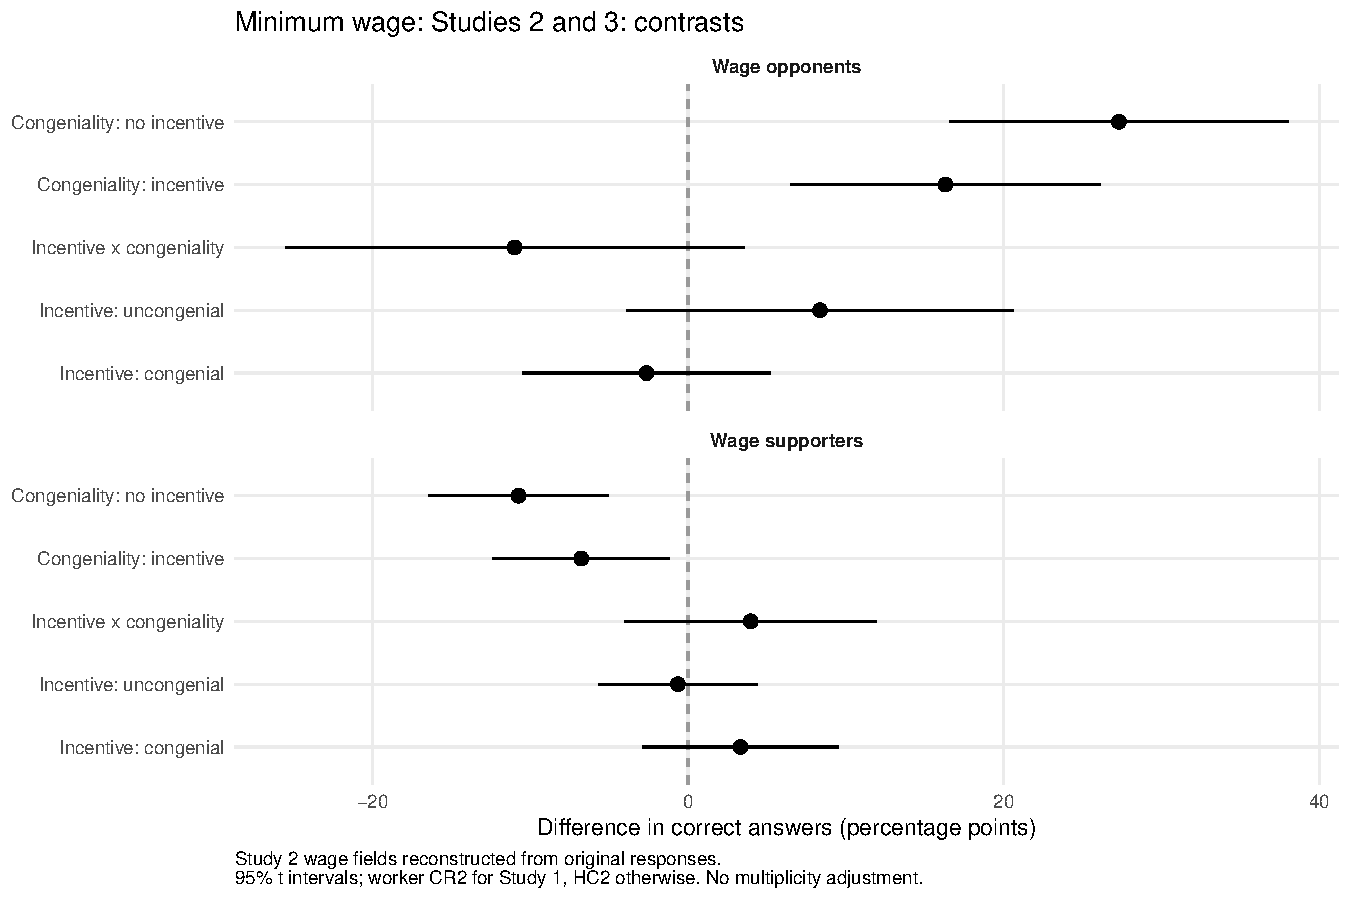
\includegraphics[width=.95\linewidth,height=.35\textheight,keepaspectratio]{../figs/figure_4_contrasts.pdf}
\caption{Minimum wage task, Studies 2 and 3. The upper plot shows correctness by condition; the lower plot shows contrasts. Groups are named in each panel. Intervals are 95\% HC2/t.}\label{fig:mwpool}
\end{figure}

Among opponents of raising the minimum wage, correctness without incentives is \result{cell.figure_4.wage_opponents.0.0.estimate.one}\% in the uncongenial condition and \result{cell.figure_4.wage_opponents.1.0.estimate.one}\% in the congenial condition. The congeniality effect falls from \result{accuracy.figure_4.wage_opponents.congeniality_no_incentive.estimate.one} to \result{accuracy.figure_4.wage_opponents.congeniality_incentive.estimate.one} points with incentives. This attenuation is imprecisely estimated: the interaction is \result{accuracy.figure_4.wage_opponents.interaction.estimate.one} points (95\% CI \result{accuracy.figure_4.wage_opponents.interaction.ci}; $p\result{accuracy.figure_4.wage_opponents.interaction.p}$). The incentive effect in the uncongenial condition is \result{accuracy.figure_4.wage_opponents.incentive_uncongenial.estimate.one} points (95\% CI \result{accuracy.figure_4.wage_opponents.incentive_uncongenial.ci}).

Supporters of raising the minimum wage do not display the predicted positive congeniality effect. In fact, the congeniality effect is \result{accuracy.figure_4.wage_supporters.congeniality_no_incentive.estimate.one} percentage points without incentives (95\% CI \result{accuracy.figure_4.wage_supporters.congeniality_no_incentive.ci}), indicating that respondents are actually {\it less} likely to correctly report a congenial result than an uncongenial result. In this case, the theoretical expectation for incentives is unclear, because the bias in the control condition is neither consistent with directionally motivated learning nor responding. We do not expect incentives to significantly alter behavior if there is no bias to reduce. Indeed, incentives do little to affect responses in either the uncongenial or congenial condition, so the congeniality effect remains negative with incentives.\footnote{
One possible explanation for this finding is that behavior in this task was affected by the previous task on concealed carry, since we did not randomize task order. We explore this possibility in SI Section~\ref{sec:spillover} but find little support for it.
Another, related possibility is that respondents mistook the row labels in the second task to be parallel to the row labels in the first task (i.e., cities enacting the given policy are always in the first row). Properly testing this hypothesis (e.g., by fully randomizing row and column labels, and task order) is beyond the scope of this study.}
Nevertheless, this finding suggests that a congeniality bias in factual learning is yet less common than the literature suggests.
In sum, across the two experimental tasks in our three studies, the patterns are consistent with motivated learning and responding, but the estimated changes in congeniality gaps are uncertain.

\subsection*{Biased Study Ratings}

Does the congeniality of the hypothetical study's result affect how positively respondents rate the study? Recall that after the concealed carry task in both Study 1 and 2, we had asked respondents to rate how ``well done'' and ``convincing'' they found the study on a 0--10 scale (see SI Section~\ref{sec:qwording} for wording). We find that the two ratings are strongly correlated, so we average them into a single rating (Cronbach's $\alpha$ = \result{rating.alpha}).

In Figure~\ref{fig:ratings}, we plot the effect of congeniality on average ratings among concealed carry supporters and opponents. The direct incentive-by-congeniality interactions are \result{rating.carry_supporters.interaction.estimate} rating points for supporters (95\% CI \result{rating.carry_supporters.interaction.ci}; $p\result{rating.carry_supporters.interaction.p}$) and \result{rating.carry_opponents.interaction.estimate} for opponents (95\% CI \result{rating.carry_opponents.interaction.ci}; $p\result{rating.carry_opponents.interaction.p}$). Pooling the groups gives an interaction of \result{rating.pooled.interaction.estimate} (95\% CI \result{rating.pooled.interaction.ci}; $p\result{rating.pooled.interaction.p}$). These positive estimates are imprecise; separate tests within incentive conditions do not establish that incentives increase the congeniality effect.

\begin{figure}[p]
\centering
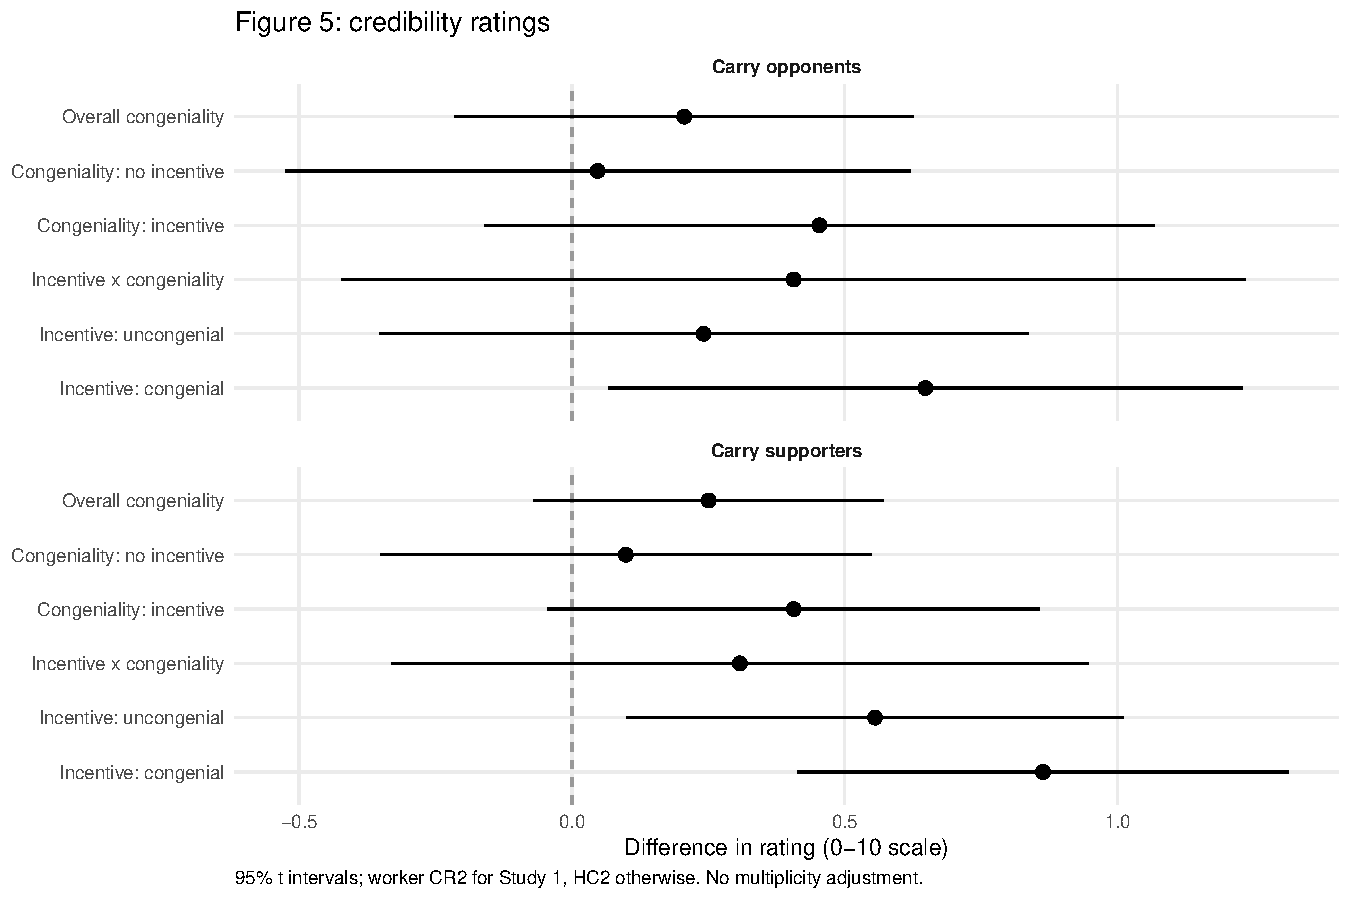
\includegraphics[width=.95\linewidth,height=.35\textheight,keepaspectratio]{../figs/figure_5.pdf}
\caption{Congeniality effects on average 0--10 study ratings, pooled Study 1 and high-numeracy Study 2. Points show effects and direct interactions; horizontal intervals are 95\% worker-cluster CR2. Study 2 records are treated as distinct workers.}\label{fig:ratings}
\end{figure}

One possible explanation for this pattern is that respondents express displeasure through study ratings when incentivized to report an uncongenial fact. Among correct respondents receiving incentives, the descriptive congeniality differences are \result{welch.0.1.true.estimate} points for concealed carry supporters and \result{welch.1.1.true.estimate} for opponents. These comparisons condition on a post-treatment outcome and do not identify that mechanism.


\section*{Discussion}

Increasing affective polarization \citep[see, e.g.,][]{iyengar2012affect, iyengar2014fear} has brought long-standing concerns over motivated reasoning to the fore. These concerns were amply highlighted during the recent presidential election, with numerous stories of people quickly latching on to congenial information, whatever the source, making the rounds. Motivated learning is related to such incidents, but it refers to something even more alarming: people coming across the same information supporting an unambiguous conclusion and yet walking away with different beliefs about what this information supports.

Motivated learning is particularly troubling because it has the potential to upend the benefits bestowed by the information age---easy access to reliable, trustworthy, objective information about a variety of politically relevant topics. Motivated learning means that people may possess different facts even after being exposed to the same information supporting an unambiguous conclusion, and may reach preferences that are very different from what they would had if they learned in an unbiased manner \citep{gilens2001, hochschild2001}. Given that motivated learning facilitates disagreement over what the facts are, it also implies that the possibility of democratic deliberation and compromise is slimmer still \citep{shapiro2008, muirhead2013}.

Our findings are consistent with motivated learning in some cases and with response processes contributing to observed congeniality gaps. Concealed carry supporters retain a congeniality gap under incentives; the design does not establish that the entire remaining gap is motivated learning. Manipulating the congeniality of the data through a minor change has a significant impact on the probability of reporting the correct answer among these respondents. We do not detect a change in this tendency under incentives. 
On the other hand, the changes in reported answers are consistent with motivated responding. When other respondents are offered a mere \$0.10 to report their beliefs accurately, estimates of motivated learning decline sharply in some cases. And given that incentives could not have affected how respondents initially processed the data---respondents could not go back and look at the data after being informed about the incentives---the response changes are consistent with motivated responding, while changes in retrieval or reasoning remain possible. 

However, there are other potential explanations for why money may reduce estimates of motivated learning. The lure of making additional money may cause respondents to choose the answer that they believe the experimenter favors, rather than the one they think is right. Or, respondents may take monetary incentives as a cue that the congenial answer is incorrect. In both cases, the decline would be artifactual. We explore both possibilities, finding little empirical support for either (see SI~\ref{sec:demand}, and in particular tables~\ref{tab:demand_opp} and~\ref{tab:demand_supp}). On balance, the data suggest that incentives reduced bias in estimates of motivated learning, rather than increase it.

It is possible that the data, even accounting for incentives, still overstate the extent to which people learn (or mislearn) in a biased manner. It is likely that a non-trivial proportion of respondents in the experimental tasks simply tune out because they find the wording too complex, or because they are disinterested in the question. Such respondents may pick an answer by taking a blind guess or by relying on their priors. They are aware that they haven not really learned the result supported by the study. Other respondents may use cheap heuristics to deduce the correct result. And some of these respondents also likely know the fallibility of inference, and prorate their certainty in what they have learned accordingly. A simple correct/incorrect scoring does not capture either of these concerns, instead treating each answer as evidence of learning a particular result. To assess these concerns, we asked people how confident they were about the answers they gave after they had selected their answers in Study 3. Among no-incentive respondents with observed correctness and confidence, \result{confidence.gun.certain}\% are certain in the concealed carry task, and \result{confidence.gun.incorrect}\% are both certain and incorrect. These joint shares describe confidence after the task; they do not measure changes from prior confidence or beliefs.\footnote{In the minimum wage task, \result{confidence.wage.certain}\% of no-incentive respondents are certain, and \result{confidence.wage.incorrect}\% are both certain and incorrect. We present these results in more detail in Table~\ref{tab:confidence} in SI Section~\ref{sec:confidence}.}

Two other pieces of evidence suggest that motivated learning is less common than what conventional estimates reveal. Firstly, we find no clear signed recall differences, although the intervals do not establish equivalence. Secondly, among those who support increasing the minimum wage, the congeniality effect is \textit{negative}---respondents were more likely to report the correct result in the uncongenial condition than in the congenial condition. This is exactly the opposite of what the theory of motivated learning would have predicted, which suggests that motivated learning may not be a feature of learning more generally.

Lastly, the minimum wage task has higher correctness, but the comparison does not isolate task difficulty: topic, presentation, and order also differ. This may happen because when the truth is transparent and easy to grasp, even people who are otherwise prone to motivated reasoning have trouble denying it \citep[see also][who shows that when economic conditions are unambiguous, as in the 2008 recession, factual beliefs about the economy converge]{bisgaard2015}. The finding is consistent with bounded rationality, a mechanism proposed for motivated learning. When little effort is required, motivated learning is perhaps not as much an issue. This also suggests that treatments designed to teach people how to infer data correctly from the contingency table ought to prove efficacious. So should treatments that give people more time to learn, and incentivize attention.

More work is, however, needed to understand why the estimated incentive effects differ between those who oppose concealed carry and those who support it. One possibility is that supporters of concealed carry have a stronger affective reaction to the issue and experience a greater directional pull toward their preferred conclusion. Another possibility is that this group of respondents differs on traits, such as need for cognition, that likely affect the extent to which people learn in a biased learning \citep[e.g.,][]{arceneaux2013}.

The estimated reductions in congeniality gaps have implications for survey measurement. It suggests that in order to precisely measure certain variables, such as factual beliefs with partisan implications, accuracy incentives may be the best way to obtain unbiased estimates. In extending this method to experiments on learning, our study contributes to the burgeoning literature on motivated responding, which combines the insights of survey satisficing with literature on group-based reasoning and affect \citep{bullock2015, prior2015}. 

To put the results in perspective, however, note that estimates of motivated learning and motivated responding come from a unique task. The task of interpreting a contingency table is unusual for many people. It is also the case that the data in the table is arranged so that common heuristics (e.g., focusing on the upper-left cell) will always lead to the wrong answer. While news media occasionally present studies using tabular or graphical formats, it is not the norm. And in such cases, it is likely that training people in how to interpret tables or incentivizing how attentively they process the data will significantly reduce bias. 

Finally, the estimated increase in the congeniality effect on study ratings is positive but imprecise. Ratings of uncongenial studies do not decline in absolute terms under incentives. Thus, these data do not establish that increased accuracy comes at the price of increased credibility bias. The possibility remains consistent with research showing that people can agree on factual information while interpreting it differently \citep[e.g.,][]{gaines2007, bisgaard2015}.

\clearpage
\bibliographystyle{../data/reference/manuscript/apa}
\bibliography{../data/reference/manuscript/partisanlearning}  
\clearpage

\clearpage
\section*{Supporting Information}
\setcounter{section}{0}
\setcounter{table}{0}
\setcounter{figure}{0}
\renewcommand\thetable{SI\arabic{table}}
\renewcommand\thefigure{SI\arabic{figure}}
\section{Additional Details about the Sample and Research Design}

\subsection{Question Wording}
\label{sec:qwording}
\singlespacing
\setlength{\parindent}{0cm} 

\subsubsection{Gun Attitudes and Ownership (Studies 1, 2, and 3)}
Do you favor or oppose a federal law requiring a nationwide ban on people other than law enforcement officers carrying concealed weapons?
\vspace{-3mm}
\begin{itemize}
\setlength\itemsep{-.5em}
  \item Ban people other than law enforcement officers from carrying concealed weapons
  \item Do not ban people other than law enforcement officers from carrying concealed weapons
  \item Unsure
\end{itemize}

How important is the issue to you?
\vspace{-3mm}
\begin{itemize}
\setlength\itemsep{-.5em}
  \item Extremely important
  \item Very important
  \item Somewhat important
  \item Not too important
  \item Not important at all
\end{itemize}

Do you or someone else in your household own a gun?
\vspace{-3mm}
\begin{itemize}
\setlength\itemsep{-.5em}
  \item Yes
  \item No
\end{itemize}

\subsubsection{Minimum Wage Attitudes (Studies 2 and 3 Only)}
The federal minimum wage is currently \$7.25 per hour. Do you favor or oppose raising the federal minimum wage?
\vspace{-3mm}
\begin{itemize}
\setlength\itemsep{-.5em}
  \item Favor raising the federal minimum wage
  \item Oppose raising the federal minimum wage
  \item Neither favor nor oppose raising the federal minimum wage
\end{itemize}

How important is the issue to you?
\vspace{-3mm}
\begin{itemize}
\setlength\itemsep{-.5em}
  \item Extremely important
  \item Very important
  \item Somewhat important
  \item Not too important
  \item Not important at all
\end{itemize}


\subsubsection{Concealed Carry Task (Studies 1, 2, and 3)}
A city government is trying to decide whether to pass a law banning private citizens from carrying concealed handguns in public. Government officials were unsure whether the law would be more likely to decrease crime by reducing the number of people carrying weapons or increase crime by making it harder for law-abiding citizens to defend themselves from violent criminals.

\medskip
Researchers completed a study of two groups of cities to answer that question. The study involved comparing changes in annual crime rates for one group of cities that \uline{had} banned concealed handguns with changes in annual crime rates for a second group of cities that had \uline{not} banned concealed handguns.

\medskip
In each group, the number of cities in which the crime rate \uline{decreased} and the number of cities in which the crime rate \uline{increased} are recorded in the table below. The exact number of cities in each group is not the same, but this does not prevent assessment of the results.

\medskip
\textbf{We would like to know whether cities that enacted a ban were more likely to have a \underline{decrease} or \underline{increase} in crime than cities without bans.}

\begin{table}[h]
\centering
\caption*{{[}Display if randomly assigned to anti-gun condition:{]}} \label{tab:siantigun_corrected}
\begin{tabular}{|l|l|l|}
\hline 
  & Increase in crime  & Decrease in crime \\\hline
  Cities that \underline{did} ban carrying     & \multirow{2}{*}{223 cities} & \multirow{2}{*}{75 cities} \\ 
  concealed handguns in public           &               & \\ \hline
  Cities that \underline{did not} ban carrying & \multirow{2}{*}{107 cities} & \multirow{2}{*}{21 cities} \\ 
  concealed handguns in public           &               &  \\\hline
\end{tabular}
\end{table}

\vspace{-5mm}
\begin{table}[h]
\centering
\caption*{{[}Display if randomly assigned to pro-gun condition:{]}} \label{tab:siprogun_corrected}
\begin{tabular}{|l|l|l|}
\hline 
  & Decrease in crime & Increase in crime \\\hline
  Cities that \underline{did} ban carrying     & \multirow{2}{*}{223 cities} & \multirow{2}{*}{75 cities} \\ 
  concealed handguns in public           &               & \\ \hline
  Cities that \underline{did not} ban carrying & \multirow{2}{*}{107 cities} & \multirow{2}{*}{21 cities} \\ 
  concealed handguns in public           &               &  \\\hline
\end{tabular}
\end{table}

\vspace{-5mm}
\begin{center}
 {[}Page Break{]}
\end{center}

What result does the study support? {[}\textbf{Incentive Treatment:}{]} We will give you a bonus of \$0.10 for the correct answer.
\begin{itemize}
  \item Cities that enacted a ban on carrying concealed handguns were more likely to have \uline{a decrease in crime} than cities without bans.
  \item Cities that enacted a ban on carrying concealed handguns were more likely to have \uline{an increase in crime} than cities without bans.
\end{itemize}

\begin{center}
{[}Page Break{]}\\
\end{center}

On a scale of 0 to 10, where 0 is ``very poorly done'' and 10 is ``very well done,'' how well do you think the study on concealed handguns was done?

\bigskip
On a scale of 0 to 10, where 0 is ``completely unconvincing'' and 10 is ``completely convincing,'' how convincing is this study as evidence of the effect of banning concealed handguns on crime?

\subsubsection{Minimum Wage Task (Studies 2 and 3 Only)}
A city government is trying to decide whether to pass a law increasing the minimum wage. Government officials were unsure whether the law would be more likely to decrease jobs or increase jobs.
 
\medskip
Researchers completed a study of two groups of states to answer that question. The study involved comparing changes in jobs for one group of states that \uline{had} increased the minimum wage with changes in jobs for a second group of states that had \uline{not} increased the minimum wage.
 
\medskip
In each group, the percentage of states in which jobs \uline{decreased} and the percentage of states in which jobs \uline{increased} are recorded in the table below. The exact number of states in each group is not the same, but this does not prevent assessment of the results.
 
\medskip
\textbf{We would like to know whether states that increased the minimum wage were more likely to have a \underline{decrease} or \underline{increase} in jobs than states without minimum wage increases.}

\begin{table}[h]
\centering
\caption*{{[}Display if randomly assigned to pro-raise condition:{]}} \label{tab:siprowage}
\begin{tabular}{|l|l|l|}
\hline 
  & Increase in jobs  & Decrease in jobs \\\hline
  States that \underline{did not} increase     & \multirow{2}{*}{16\%} & \multirow{2}{*}{84\%} \\ 
  minimum wage           &               & \\ \hline
  States that \underline{did} increase & \multirow{2}{*}{37\%} & \multirow{2}{*}{63\%} \\ 
  minimum wage           &               &  \\\hline
\end{tabular}
\end{table}

\vspace{-5mm}
\begin{table}[h]
\centering
\caption*{{[}Display if randomly assigned to anti-raise condition:{]}} \label{tab:siantiwage}
\begin{tabular}{|l|l|l|}
\hline 
  & Increase in jobs  & Decrease in jobs \\\hline
  States that \underline{did} increase     & \multirow{2}{*}{16\%} & \multirow{2}{*}{84\%} \\ 
  minimum wage           &               & \\ \hline
  States that \underline{did not} increase & \multirow{2}{*}{37\%} & \multirow{2}{*}{63\%} \\ 
  minimum wage           &               &  \\\hline
\end{tabular}
\end{table}

\vspace{-2.5mm}
\begin{center}
 {[}Page Break{]}
\end{center}

What result does the study support? {[}\textbf{Incentive Treatment:}{]} We will give you a bonus of \$0.10 for the correct answer.
\begin{itemize}
  \item States that increased the minimum wage were more likely to have \uline{a decrease in jobs} than states without minimum wage increases.
  \item States that increased the minimum wage were more likely to have \uline{an increase in jobs} than states without minimum wage increases.
\end{itemize}

\bigskip
\subsection{Numeracy Screener}
\label{sec:numscreener}
\doublespacing
\setlength{\parindent}{1cm} 

We include our numeracy scale below. It is a shortened version of the scale used by \citet{kahan2017} and developed by \citet{weller2012}. We include the five easiest items that \citeauthor{weller2012} find, in order to identify low-numeracy respondents. Two concerns vitiate commensurability of our scores and those of \citeauthor{kahan2017}: guessing and item sampling. Research suggests that lucky guessing is a minor concern on open-ended items \citep{luskin2011}. And if we assume that the items are Guttman scaled, i.e., a person who answers a more difficult item correctly will also answer easier items correctly, our threshold will be exactly the same as the median score in \citeauthor{kahan2017}. We take Guttman scaling on numeracy items to not only be plausible but likely.

\begin{enumerate}
  \item If we roll a fair, six-sided die 1,000 times, on average, how many times would the die come up as an even number? \\{\bf Answer:} 500
  \item There is a 1\% chance of winning a \$10 prize in the Megabucks Lottery. On average, how many people would win the \$10 prize if 1,000 people each bought a single ticket? \\{\bf Answer:} 10
  \item If the chance of getting a disease is 20 out of 100, this would be the same as having a \underline{\hspace{1cm}}\% chance of getting the disease. \\{\bf Answer:} 20
  \item If there is a 10\% chance of winning a concert ticket, how many people out of 1,000 would be expected to win the ticket? \\{\bf Answer:} 100
  \item In the PCH Sweepstakes, the chances of winning a car are 1 in a 1,000. What percent of PCH Sweepstakes tickets win a car? \\{\bf Answer:} .1
\end{enumerate}

\newpage
\subsection{Respondents Enrolled, Screened, Allocated, and Analyzed by Study}
\label{sec:flow}
Figures~\ref{fig:flowchart1},~\ref{fig:flowchart2}, and~\ref{fig:flowchart3} display source survey counts, released records, observed answers, and policy-position subsets. Counts overlap and are not a sequence of exclusions. Study 1 records include repeated workers; Study 2 records are assumed to represent distinct workers.

\bigskip
\begin{figure}[p]
\centering
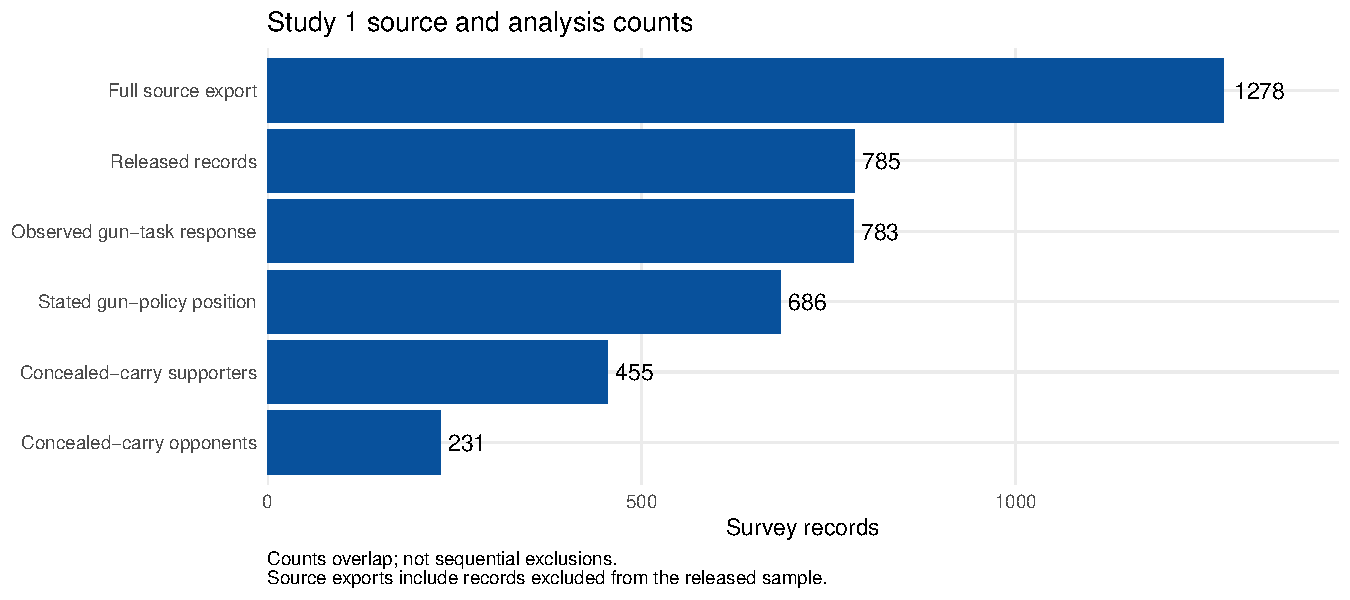
\includegraphics[width=.95\linewidth,height=.34\textheight,keepaspectratio]{../figs/figure_si_1.pdf}
\caption{Study 1 source and analysis counts. Counts overlap; they are not sequential exclusions.}\label{fig:flowchart1}
\end{figure}

\begin{figure}[p]
\centering
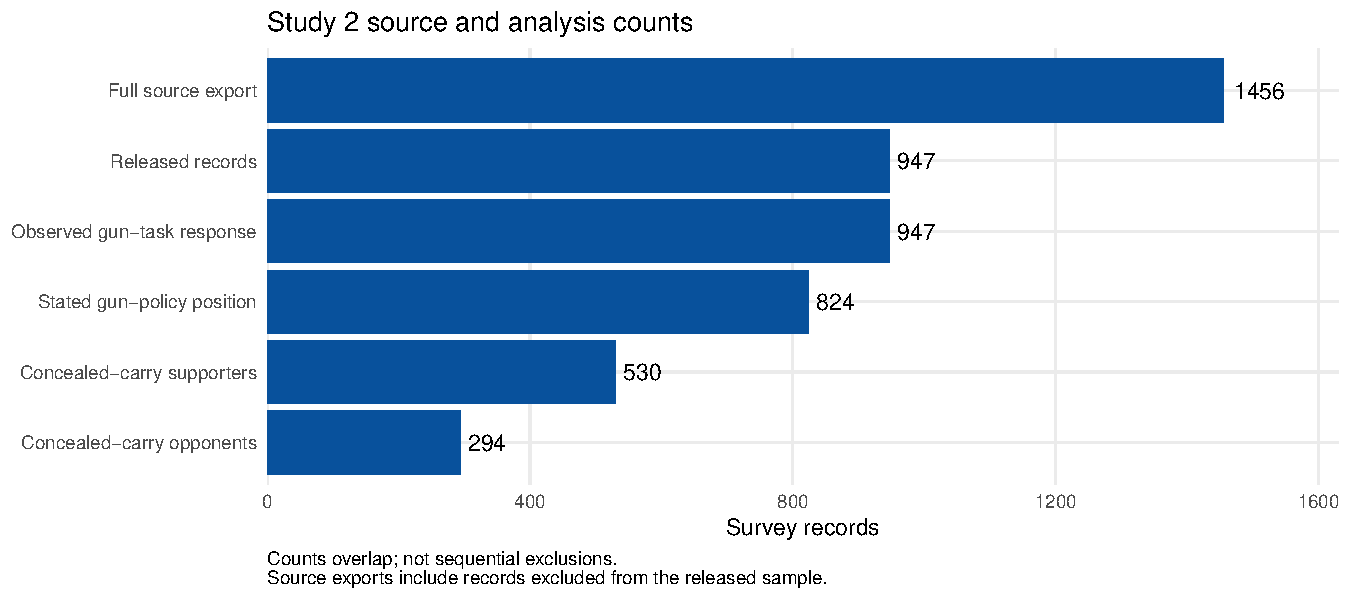
\includegraphics[width=.95\linewidth,height=.34\textheight,keepaspectratio]{../figs/figure_si_2.pdf}
\caption{Study 2 source and analysis counts. Counts overlap; they are not sequential exclusions.}\label{fig:flowchart2}
\end{figure}

\begin{figure}[p]
\centering
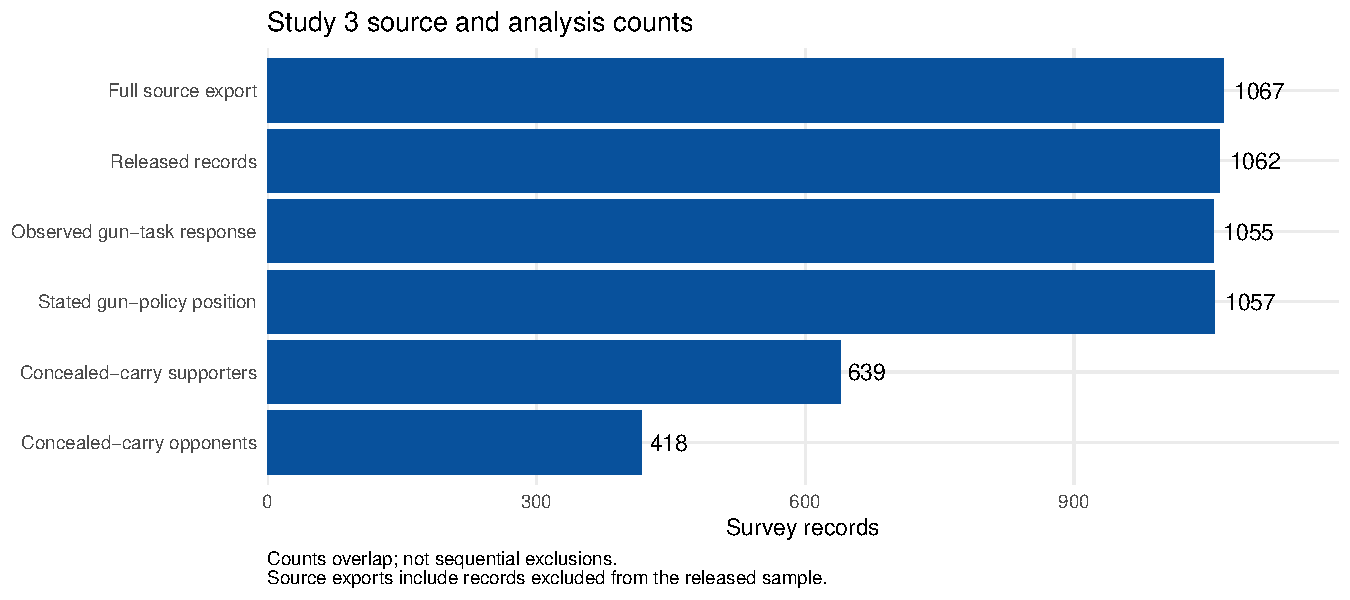
\includegraphics[width=.95\linewidth,height=.34\textheight,keepaspectratio]{../figs/figure_si_3.pdf}
\caption{Study 3 source and analysis counts. Counts overlap; they are not sequential exclusions.}\label{fig:flowchart3}
\end{figure}

\clearpage
\subsection{Sample Characteristics}
\label{sec:sample}

Table~\ref{tab:sample} reports sample characteristics calculated from the reconstructed data. The original supplement also reports national benchmarks from the 2012 American National Election Study and 2015 American Community Survey; those comparisons remain available in the preserved source materials. High numeracy means at least four correct items on the five-item scale. This group contains \result{sample.2.high} records (\result{sample.2.high_pct}\%) in Study 2 and \result{sample.3.high} (\result{sample.3.high_pct}\%) in Study 3. High-numeracy respondents in Study 3 are more educated, white, and male than the full sample.

\singlespacing
\begingroup\footnotesize\singlespacing

\begin{longtable}[t]{lllllll}
\caption{\label{tab:sample}Sample characteristics}\\
\toprule
Characteristic & Category & Study 1 & Study 2 & Study 2: high & Study 3 & Study 3: high\\
\midrule
\endfirsthead
\toprule
Characteristic & Category & Study 1 & Study 2 & Study 2: high & Study 3 & Study 3: high\\
\midrule
\endhead
Party & Democrat & 65.1 (511) & 61.0 (578) & 62.6 (433) & 50.6 (536) & 49.4 (208)\\
Party & Independent & 14.0 (110) & 15.9 (151) & 15.9 (110) & 14.1 (149) & 11.6 (49)\\
Party & Republican & 20.9 (164) & 23.0 (218) & 21.5 (149) & 35.3 (374) & 39.0 (164)\\
Ideology & Conservative & 16.2 (127) & 16.8 (159) & 15.5 (107) & 28.5 (302) & 28.3 (119)\\
Ideology & Liberal & 50.5 (396) & 50.3 (475) & 52.0 (359) & 23.3 (246) & 22.1 (93)\\
Ideology & Moderate & 33.3 (261) & 32.9 (311) & 32.5 (224) & 48.2 (510) & 49.6 (209)\\
Education & College Degree & 39.9 (313) & 38.7 (366) & 39.5 (273) & 26.4 (279) & 33.0 (139)\\
Education & HS or Less & 9.1 (71) & 11.7 (111) & 9.8 (68) & 25.1 (266) & 17.1 (72)\\
Education & Post-Graduate & 10.7 (84) & 8.8 (83) & 10.1 (70) & 9.9 (105) & 13.1 (55)\\
Education & Some College & 40.3 (316) & 40.8 (386) & 40.5 (280) & 38.6 (408) & 36.8 (155)\\
Age & 18-29 & 58.9 (462) & 49.3 (466) & 48.9 (338) & 9.8 (104) & 10.9 (46)\\
Age & 30-44 & 31.5 (247) & 37.7 (357) & 39.5 (273) & 33.9 (358) & 32.5 (137)\\
Age & 45-64 & 9.0 (71) & 11.6 (110) & 10.4 (72) & 43.6 (460) & 46.8 (197)\\
Age & 65 or older & 0.6 (5) & 1.4 (13) & 1.2 (8) & 12.7 (134) & 9.7 (41)\\
Sex & Male & 67.6 (531) & 61.9 (586) & 66.3 (458) & 33.9 (358) & 43.1 (181)\\
Sex & Female & 32.4 (254) & 38.1 (360) & 33.7 (233) & 66.1 (698) & 56.9 (239)\\
Race/ethnicity & Asian, Non-Hisp & 10.6 (83) & 9.5 (90) & 10.9 (75) & 2.9 (30) & 4.1 (17)\\
Race/ethnicity & Black, Non-Hisp & 4.6 (36) & 6.1 (58) & 5.1 (35) & 10.5 (110) & 5.0 (21)\\
Race/ethnicity & Hispanic/Latino & 5.2 (41) & 6.8 (64) & 6.7 (46) & 6.8 (72) & 3.8 (16)\\
Race/ethnicity & Mixed & 3.6 (28) & 3.8 (36) & 3.9 (27) & 2.1 (22) & 1.4 (6)\\
Race/ethnicity & Other, Non-Hisp & 0.6 (5) & 1.2 (11) & 0.7 (5) & 1.3 (14) & 1.2 (5)\\
Race/ethnicity & White, Non-Hisp & 75.4 (590) & 72.6 (686) & 72.8 (502) & 76.4 (804) & 84.4 (353)\\
\bottomrule
\end{longtable}
\noindent\footnotesize Percent of nonmissing responses, with counts in parentheses. High numeracy means at least four correct items.\par\normalsize

\endgroup
\doublespacing

\clearpage
\subsection{Covariate Balance}
\label{sec:balance}

Table~\ref{tab:balance} reports classical F tests for the historical balance specifications. Studies 1 and 2 use congeniality, incentives, and their interaction except for race, which uses incentives alone; Study 3 uses incentives alone. N is the complete-case sample for each model. Alternative race specifications are provided in the replication tables. These comparisons do not establish that randomization was implemented correctly.

\vspace{-3mm}
\singlespacing
\begingroup\footnotesize\singlespacing

\begin{longtable}[t]{rlrrrrl}
\caption{\label{tab:balance}Covariate balance}\\
\toprule
Study & Outcome & N & F & df1 & df2 & p\\
\midrule
\endfirsthead
\toprule
Study & Outcome & N & F & df1 & df2 & p\\
\midrule
\endhead
1 & party id & 686 & 0.44 & 3 & 682 & 0.727\\
1 & ideology & 685 & 0.30 & 3 & 681 & 0.828\\
1 & education code & 685 & 2.42 & 3 & 681 & 0.065\\
1 & age years & 686 & 1.23 & 3 & 682 & 0.297\\
1 & is female & 686 & 1.53 & 3 & 682 & 0.204\\
1 & is white & 783 & 0.64 & 1 & 781 & 0.424\\
2 & party id & 824 & 0.76 & 3 & 820 & 0.519\\
2 & ideology & 822 & 1.29 & 3 & 818 & 0.275\\
2 & education code & 823 & 0.78 & 3 & 819 & 0.505\\
2 & age years & 824 & 0.56 & 3 & 820 & 0.643\\
2 & is female & 823 & 0.47 & 3 & 819 & 0.706\\
2 & is white & 945 & 1.40 & 1 & 943 & 0.238\\
3 & party id & 1055 & 0.08 & 1 & 1053 & 0.784\\
3 & ideology & 1055 & 0.00 & 1 & 1053 & 0.961\\
3 & education code & 1055 & 2.51 & 1 & 1053 & 0.113\\
3 & age years & 1053 & 1.00 & 1 & 1051 & 0.317\\
3 & is female & 1053 & 1.04 & 1 & 1051 & 0.309\\
3 & is white & 1049 & 0.06 & 1 & 1047 & 0.810\\
\bottomrule
\end{longtable}
\noindent\footnotesize Classical F tests. Studies 1 and 2 use policy-congeniality factorials except race, which uses incentives alone. Study 3 uses incentives alone. Alternative race specifications are in race\_balance\_checks.csv.\par\normalsize

\endgroup
\doublespacing

%\clearpage
\vspace{-5mm}
\subsection{Assessing Spillover}
\label{sec:spillover}

Because the concealed carry task always preceded the minimum wage task in Studies 2 and 3, we assess the extent to which randomization in the former task affected behavior in the latter task. We estimate treatment effects in both tasks simultaneously via logistic regression. The outcome variable indicates correctness in the minimum wage task (1 = correct). The regressors are the congeniality treatment, the incentive treatment, and their interaction, in both tasks. We allow the minimum wage treatments to vary by concealed carry condition.

Table~\ref{tab:spillover} displays results for wage supporters in Studies 2 and 3 and opponents in Study 3. The reconstructed Study 2 model has full factorial rank. Sample sizes and coefficients are taken directly from the fitted models. Individual first-task coefficients provide no clear evidence of spillover, but these tests do not establish its absence. Because task order was fixed, they also do not identify the effect of reversing task order.

\medskip
\begingroup\footnotesize\singlespacing

\begin{longtable}[t]{lllrrlrr}
\caption{\label{tab:spillover}Wage correctness and cross-task assignments}\\
\toprule
Model & Term & Covariance & Estimate & SE & p & N & OR\\
\midrule
\endfirsthead
\toprule
Model & Term & Covariance & Estimate & SE & p & N & OR\\
\midrule
\endhead
Wage 2:1 & Intercept & classical & 1.558 & 0.389 & <0.001 & 613 & 4.750\\
Wage 2:1 & GC & classical & 0.611 & 0.656 & 0.351 & 613 & 1.842\\
Wage 2:1 & GI & classical & 0.777 & 0.719 & 0.280 & 613 & 2.175\\
Wage 2:1 & WC & classical & 0.927 & 0.716 & 0.195 & 613 & 2.526\\
Wage 2:1 & WI & classical & 1.045 & 0.830 & 0.208 & 613 & 2.842\\
Wage 2:1 & GC:GI & classical & 0.717 & 1.349 & 0.595 & 613 & 2.049\\
Wage 2:1 & GC:WC & classical & -1.767 & 0.965 & 0.067 & 613 & 0.171\\
Wage 2:1 & GI:WC & classical & -1.443 & 1.035 & 0.163 & 613 & 0.236\\
Wage 2:1 & GC:WI & classical & 0.450 & 1.412 & 0.750 & 613 & 1.568\\
Wage 2:1 & GI:WI & classical & -1.534 & 1.117 & 0.169 & 613 & 0.216\\
Wage 2:1 & WC:WI & classical & -0.667 & 1.256 & 0.595 & 613 & 0.513\\
Wage 2:1 & GC:GI:WC & classical & -0.157 & 1.627 & 0.923 & 613 & 0.855\\
Wage 2:1 & GC:GI:WI & classical & -1.545 & 1.964 & 0.432 & 613 & 0.213\\
Wage 2:1 & GC:WC:WI & classical & -0.735 & 1.789 & 0.681 & 613 & 0.480\\
Wage 2:1 & GI:WC:WI & classical & 1.209 & 1.618 & 0.455 & 613 & 3.352\\
Wage 2:1 & GC:GI:WC:WI & classical & 2.856 & 2.458 & 0.245 & 613 & 17.387\\
Wage 3:0 & Intercept & classical & 0.211 & 0.326 & 0.517 & 369 & 1.235\\
Wage 3:0 & GI & classical & 0.482 & 0.462 & 0.297 & 369 & 1.619\\
Wage 3:0 & WC & classical & 2.519 & 0.679 & <0.001 & 369 & 12.413\\
Wage 3:0 & WI & classical & 0.792 & 0.480 & 0.099 & 369 & 2.208\\
Wage 3:0 & GI:WC & classical & -1.015 & 0.920 & 0.270 & 369 & 0.363\\
Wage 3:0 & GI:WI & classical & -0.846 & 0.647 & 0.191 & 369 & 0.429\\
Wage 3:0 & WC:WI & classical & -1.443 & 0.900 & 0.109 & 369 & 0.236\\
Wage 3:0 & GI:WC:WI & classical & 0.889 & 1.182 & 0.452 & 369 & 2.432\\
Wage 3:1 & Intercept & classical & 1.655 & 0.303 & <0.001 & 683 & 5.231\\
Wage 3:1 & GI & classical & -0.060 & 0.421 & 0.888 & 683 & 0.942\\
Wage 3:1 & WC & classical & -0.961 & 0.376 & 0.011 & 683 & 0.382\\
Wage 3:1 & WI & classical & -0.032 & 0.414 & 0.939 & 683 & 0.969\\
Wage 3:1 & GI:WC & classical & 0.155 & 0.535 & 0.772 & 683 & 1.167\\
Wage 3:1 & GI:WI & classical & -0.032 & 0.577 & 0.956 & 683 & 0.969\\
Wage 3:1 & WC:WI & classical & 0.452 & 0.531 & 0.394 & 683 & 1.572\\
Wage 3:1 & GI:WC:WI & classical & -0.348 & 0.750 & 0.642 & 683 & 0.706\\
\bottomrule
\end{longtable}
\noindent\footnotesize GC/GI: gun congeniality/incentive; WC/WI: wage congeniality/incentive. Models identify study and wage support (1=yes). Coefficients are log odds; OR: odds ratio. Colons denote interactions. N is the fitted complete-case sample.\par\normalsize

\endgroup
\normalsize
\doublespacing

\clearpage
\doublespacing
\section{Additional Empirical Results}

\subsection{Does Numeracy Condition Treatment Effects?}
\label{sec:numeracy}
\doublespacing

We confined Study 1 to high-numeracy respondents based on the theoretical argument and main result of \citet{kahan2017} that polarization only occurs among this group. However, in Studies 2 and 3, we invited all respondents to participate fully, regardless of numeracy, to compare the behavior and background characteristics of high- and low-numeracy respondents. In theory, respondents may differ by numeracy in multiple ways. First, high-numeracy respondents are probably more educated, which we see in Study 3 (see Table~\ref{tab:sample}). Second, they may hold different attitudes. For example, high-numeracy respondents may exhibit greater political sophistication, ideological constraint, party identification, or other traits that predispose them to motivated learning, motivated responding, or both.

Table~\ref{tab:accnum} compares incentive effects in the concealed carry task by study, congeniality, and numeracy. Effects are percentage-point differences between incentive and no-incentive conditions, with two-sided 95\% intervals and fitted sample sizes. Study 1 includes only high-numeracy respondents. Estimated effects vary across groups, but most intervals are wide. In particular, the positive effect among low-numeracy concealed carry opponents in Study 3 does not exclude zero under two-sided inference.

\singlespacing
\begingroup\footnotesize\singlespacing

\begin{longtable}[t]{rllrrllr}
\caption{\label{tab:accnum}Incentive effects by numeracy and congeniality}\\
\toprule
Study & Numeracy & Group & Congenial & Effect & 95\% interval & p & N\\
\midrule
\endfirsthead
\toprule
Study & Numeracy & Group & Congenial & Effect & 95\% interval & p & N\\
\midrule
\endhead
1 & high & Carry opponents & 0 & 9.07 & {}[-8.73, 26.87] & 0.315 & 123\\
1 & high & Carry opponents & 1 & -7.99 & {}[-27.05, 11.06] & 0.407 & 108\\
1 & high & Carry supporters & 0 & -1.51 & {}[-13.87, 10.84] & 0.809 & 248\\
1 & high & Carry supporters & 1 & -3.30 & {}[-16.91, 10.31] & 0.633 & 207\\
2 & all & Carry opponents & 0 & 17.08 & {}[0.91, 33.26] & 0.039 & 146\\
2 & all & Carry opponents & 1 & -0.28 & {}[-16.66, 16.11] & 0.974 & 148\\
2 & all & Carry supporters & 0 & 0.61 & {}[-11.60, 12.81] & 0.922 & 252\\
2 & all & Carry supporters & 1 & 5.86 & {}[-5.98, 17.70] & 0.331 & 278\\
2 & high & Carry opponents & 0 & 25.40 & {}[6.63, 44.16] & 0.008 & 108\\
2 & high & Carry opponents & 1 & 4.01 & {}[-14.60, 22.62] & 0.670 & 117\\
2 & high & Carry supporters & 0 & -4.15 & {}[-18.71, 10.41] & 0.574 & 180\\
2 & high & Carry supporters & 1 & 2.81 & {}[-11.21, 16.82] & 0.693 & 200\\
2 & low & Carry opponents & 0 & -10.14 & {}[-43.50, 23.21] & 0.541 & 38\\
2 & low & Carry opponents & 1 & -14.96 & {}[-53.05, 23.14] & 0.428 & 31\\
2 & low & Carry supporters & 0 & 13.29 & {}[-9.52, 36.09] & 0.249 & 72\\
2 & low & Carry supporters & 1 & 13.29 & {}[-8.96, 35.54] & 0.238 & 78\\
3 & all & Carry opponents & 0 & 6.93 & {}[-1.81, 15.68] & 0.120 & 416\\
3 & all & Carry supporters & 0 & -0.31 & {}[-7.66, 7.03] & 0.933 & 639\\
3 & high & Carry opponents & 0 & 4.45 & {}[-10.58, 19.49] & 0.559 & 159\\
3 & high & Carry supporters & 0 & 2.93 & {}[-8.50, 14.36] & 0.614 & 261\\
3 & low & Carry opponents & 0 & 7.99 & {}[-2.71, 18.69] & 0.143 & 257\\
3 & low & Carry supporters & 0 & -2.41 & {}[-12.04, 7.21] & 0.622 & 378\\
\bottomrule
\end{longtable}
\noindent\footnotesize Effects are percentage points. Two-sided 95\% t intervals; Study 1 worker CR2, otherwise HC2. High numeracy: at least four correct items.\par\normalsize

\endgroup
\doublespacing

Since numeracy is not a prerequisite for understanding which result is more congenial, we also examined the odds of choosing a congenial rather than uncongenial answer among concealed carry opponents. In Study 2, these odds without incentives are \result{odds.study_2_low.carry_opponents.0.response_odds} for low-numeracy respondents and \result{odds.study_2_high.carry_opponents.0.response_odds} for high-numeracy respondents. With incentives, the corresponding odds are \result{odds.study_2_low.carry_opponents.1.response_odds} and \result{odds.study_2_high.carry_opponents.1.response_odds}. These are descriptive odds, not probability differences.

Among Study 3 concealed carry opponents, the odds of choosing a congenial answer fall from \result{odds.study_3_low.carry_opponents.0.response_odds} to \result{odds.study_3_low.carry_opponents.1.response_odds} for low-numeracy respondents, and from \result{odds.study_3_high.carry_opponents.0.response_odds} to \result{odds.study_3_high.carry_opponents.1.response_odds} for high-numeracy respondents. Low-numeracy respondents display greater descriptive response bias in both conditions.

\clearpage
\subsection{Subsetting Respondents by ``Ideological Worldview''}
\label{sec:kahan}
\doublespacing

\citet{kahan2017} operationalize congeniality using respondents' ``ideological worldview'' instead of their position on concealed carry. The authors conceive of ideological worldview as a combination of partisanship and ideology, and measure it by simply multiplying the two. At one end of the scale are ``Conservative Republicans,'' and at the other end, ``Liberal Democrats.'' And while we are skeptical, it is possible that ideological worldview establishes what information is congenial to a respondent, more so than relevant attitudes. To explore this concern, we construct a similar variable, categorizing respondents as either conservative Republicans or liberal Democrats, depending on their self reported party identification (including leaners) and three-point ideology (conservative, moderate, or liberal). Using this variable, we re-analyze the concealed carry task in Study 1 and high-numeracy Study 2.  

Before we present the results, a caveat: positions on concealed carry are only weakly related to ideological worldview, especially among low-numeracy respondents. In Study 2, for example, the correlation is \result{worldview.study_2.high.correlation} among high-numeracy respondents and \result{worldview.study_2.low.correlation} among low-numeracy respondents. In fact, this weak relationship may be why \citeauthor{kahan2017} do not observe bias among low-numeracy respondents. We prefer to subset respondents by their issue position, precisely because the overlap between issue positions and ideological worldview is not 100\%.

We recode congeniality relative to ideological worldview and present the results in Figure~\ref{fig:libdem}. Among conservative Republicans, the congeniality effects are \result{accuracy.figure_si_4.conservative_republican.congeniality_no_incentive.estimate.one} points without incentives and \result{accuracy.figure_si_4.conservative_republican.congeniality_incentive.estimate.one} with incentives. Their difference is \result{accuracy.figure_si_4.conservative_republican.interaction.estimate.one} points (95\% CI \result{accuracy.figure_si_4.conservative_republican.interaction.ci}). Among liberal Democrats, the corresponding effects are \result{accuracy.figure_si_4.liberal_democrat.congeniality_no_incentive.estimate.one} and \result{accuracy.figure_si_4.liberal_democrat.congeniality_incentive.estimate.one} points, with an interaction of \result{accuracy.figure_si_4.liberal_democrat.interaction.estimate.one} (95\% CI \result{accuracy.figure_si_4.liberal_democrat.interaction.ci}). Neither interaction excludes zero. This coding answers a different question from policy congeniality.

\begin{figure}[p]
\centering
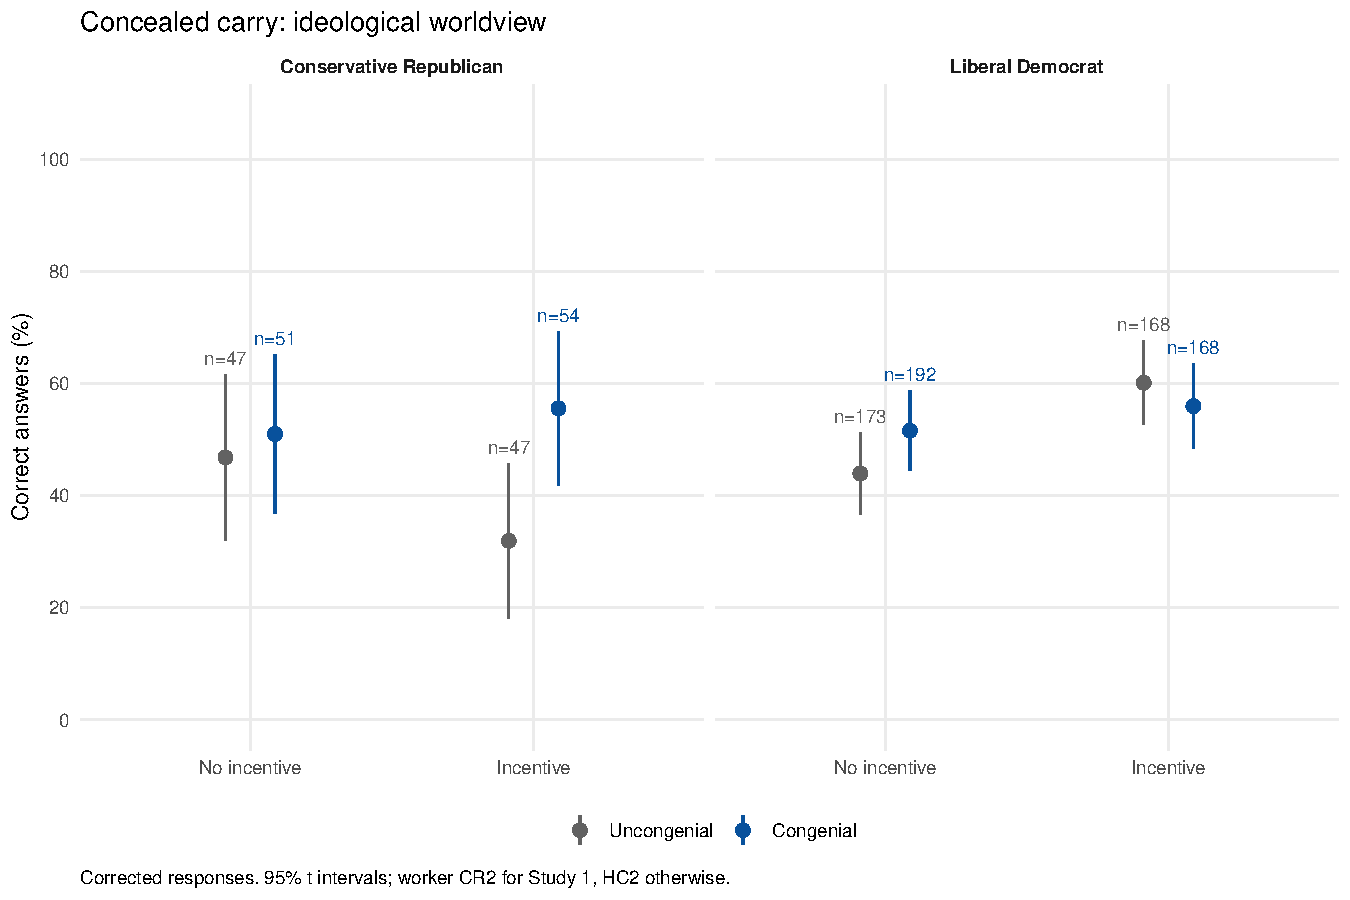
\includegraphics[width=.95\linewidth,height=.34\textheight,keepaspectratio]{../figs/figure_si_4.pdf}
\par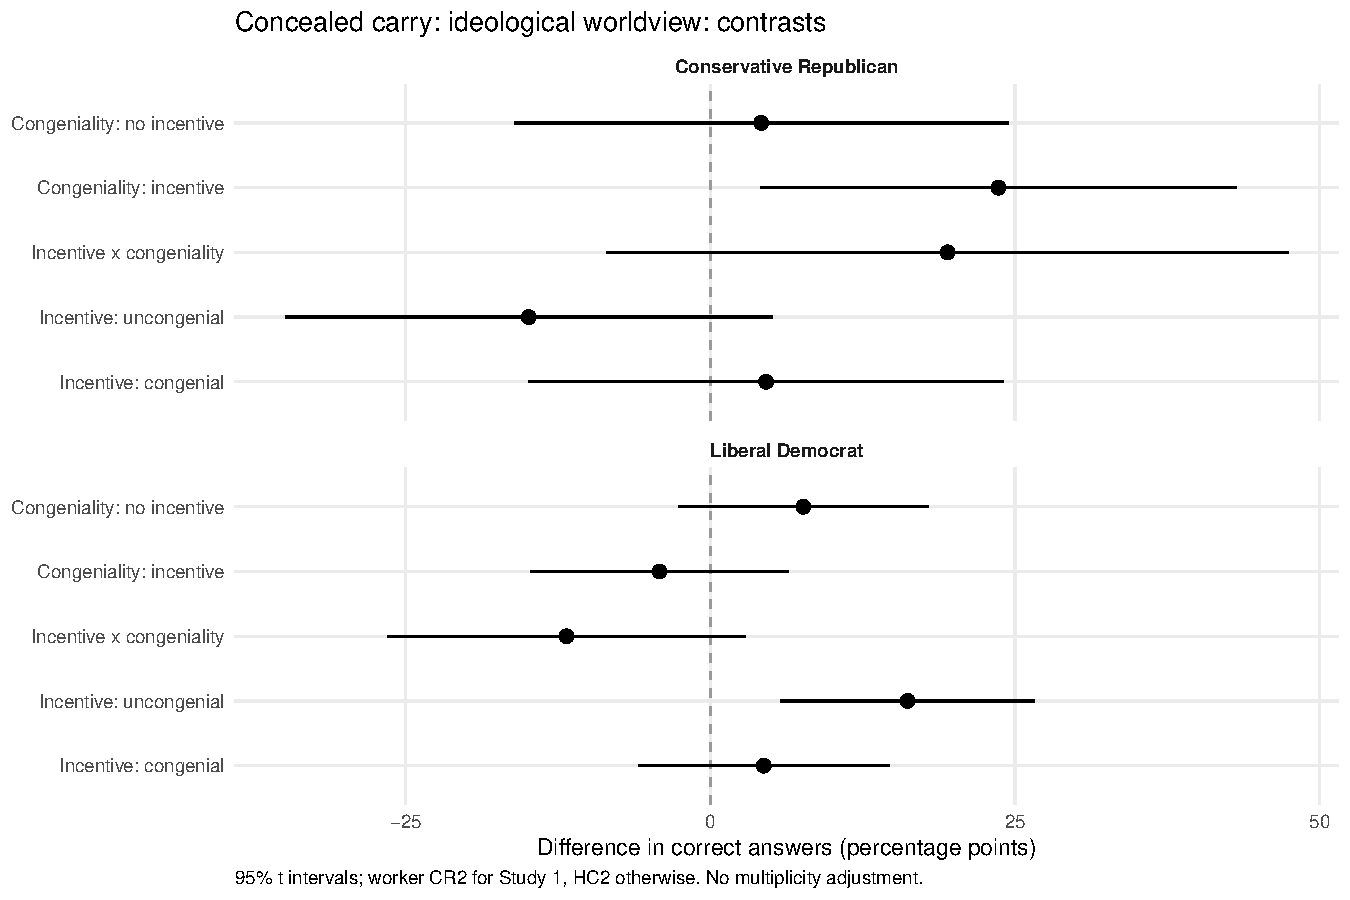
\includegraphics[width=.95\linewidth,height=.34\textheight,keepaspectratio]{../figs/figure_si_4_contrasts.pdf}
\caption{Concealed carry correctness by ideological worldview, Study 1 and high-numeracy Study 2. Upper: correctness by condition. Lower: treatment contrasts. Groups are named in each panel. Intervals are 95\% t intervals, with worker-cluster CR2 for Study 1 samples and HC2 otherwise.}\label{fig:libdem}
\end{figure}

\clearpage
\subsection{Recall of the Stimulus Data}
\label{sec:recall}

One proposed mechanism for why people learn in a motivated manner is that they simply misperceive or misremember the actual data. Thus, we next examine the extent to which errors in cognition are explained by congeniality of the data. Given our hypothesis that motivated responding explains a large portion of what appears to be motivated learning, we also conjectured that most respondents do not perceive data in a selective manner.

To test this hypothesis, we examined how well respondents did across various conditions in recalling the numbers in the contingency table (in Study 1 only). Prior studies using similar tasks suggest that errors are most common in the top-left cell in the contingency table \citep{gilovich1991, dawson2002cella}. We therefore first examine whether the congeniality manipulation changed estimates of the number of cities in this cell. Since the incentive treatment occurred only after respondents saw the contingency table, we do not expect incentives to affect recall. We therefore focus on the effect of congeniality on data recall in the absence of incentives. 

There were always 223 cities in the upper-left cell. If respondents misperceive or misremember this value in a way that makes the study's result more congenial, then we would expect them to overestimate this number in the uncongenial condition, relative to the congenial condition. Overestimating the upper-left cell inflates the crime increase:decrease (decrease:increase) ratio for cities that banned concealed handguns in the anti-gun (pro-gun) version of the table. The estimated mean difference is small. The mean was \result{recall.recall_a.0.estimate.one} (s.e. = \result{recall.recall_a.0.std_error.one}) in the uncongenial condition and \result{recall.recall_a.1.estimate.one} (s.e. = \result{recall.recall_a.1.std_error.one}) in the congenial condition (without incentives).

We next checked whether estimates of the 107 cities in the lower-left cell varied by condition. Here we would expect estimates to be {\it lower} in the uncongenial condition than in the congenial condition. However, recall was again fairly consistent across conditions: \result{recall.recall_c.0.estimate.one} (s.e. = \result{recall.recall_c.0.std_error.one}) and \result{recall.recall_c.1.estimate.one} (s.e. = \result{recall.recall_c.1.std_error.one}) in the uncongenial and congenial conditions, respectively. The other two cells also show no clear congeniality differences. In summary, we do not find a congeniality effect on the recall task in the absence of incentives.

Finally, we estimate the effects of congeniality, incentives, and their interaction on recalled counts. Tables~\ref{tab:recalla} and~\ref{tab:recallc} show classical, HC3, and worker-cluster CR2 uncertainty. The estimates provide no clear evidence of signed recall differences. They do not establish equivalent recall or rule out selective perception, retrieval, or reasoning. These regressions model recalled counts, not absolute recall error.

\vspace{5mm}
\begingroup\footnotesize\singlespacing

\begin{longtable}[t]{lllrrlr}
\caption{\label{tab:recalla}Recall of stimulus cell A}\\
\toprule
Model & Term & Covariance & Estimate & SE & p & N\\
\midrule
\endfirsthead
\toprule
Model & Term & Covariance & Estimate & SE & p & N\\
\midrule
\endhead
Recall a & Intercept & classical & 213.923 & 5.583 & <0.001 & 664\\
Recall a & GC & classical & -1.385 & 8.083 & 0.864 & 664\\
Recall a & GI & classical & -1.918 & 7.974 & 0.810 & 664\\
Recall a & GC:GI & classical & 2.662 & 11.794 & 0.822 & 664\\
Recall a & Intercept & hc3 & 213.923 & 5.547 & <0.001 & 664\\
Recall a & GC & hc3 & -1.385 & 7.417 & 0.852 & 664\\
Recall a & GI & hc3 & -1.918 & 7.663 & 0.802 & 664\\
Recall a & GC:GI & hc3 & 2.662 & 12.169 & 0.827 & 664\\
Recall a & Intercept & cr2 & 213.923 & 5.532 & <0.001 & 664\\
Recall a & GC & cr2 & -1.385 & 7.395 & 0.852 & 664\\
Recall a & GI & cr2 & -1.918 & 7.635 & 0.802 & 664\\
Recall a & GC:GI & cr2 & 2.662 & 12.123 & 0.826 & 664\\
\bottomrule
\end{longtable}
\noindent\footnotesize GC/GI: gun congeniality/incentive. Coefficients are recalled counts. Covariance identifies the inference method. Colons denote interactions. N is the fitted complete-case sample.\par\normalsize

\endgroup

\begingroup\footnotesize\singlespacing

\begin{longtable}[t]{lllrrlr}
\caption{\label{tab:recallc}Recall of stimulus cell C}\\
\toprule
Model & Term & Covariance & Estimate & SE & p & N\\
\midrule
\endfirsthead
\toprule
Model & Term & Covariance & Estimate & SE & p & N\\
\midrule
\endhead
Recall c & Intercept & classical & 103.087 & 3.397 & <0.001 & 665\\
Recall c & GC & classical & 2.099 & 4.910 & 0.669 & 665\\
Recall c & GI & classical & 1.077 & 4.851 & 0.824 & 665\\
Recall c & GC:GI & classical & 1.917 & 7.170 & 0.789 & 665\\
Recall c & Intercept & hc3 & 103.087 & 2.676 & <0.001 & 665\\
Recall c & GC & hc3 & 2.099 & 5.411 & 0.698 & 665\\
Recall c & GI & hc3 & 1.077 & 3.961 & 0.786 & 665\\
Recall c & GC:GI & hc3 & 1.917 & 7.263 & 0.792 & 665\\
Recall c & Intercept & cr2 & 103.087 & 2.668 & <0.001 & 665\\
Recall c & GC & cr2 & 2.099 & 5.396 & 0.697 & 665\\
Recall c & GI & cr2 & 1.077 & 3.952 & 0.785 & 665\\
Recall c & GC:GI & cr2 & 1.917 & 7.232 & 0.791 & 665\\
\bottomrule
\end{longtable}
\noindent\footnotesize GC/GI: gun congeniality/incentive. Coefficients are recalled counts. Covariance identifies the inference method. Colons denote interactions. N is the fitted complete-case sample.\par\normalsize

\endgroup

%\clearpage
\subsection{Covariance Detection Task Results  by Study}
\label{sec:bystudy}

Figures~\ref{fig:study1} and~\ref{fig:study2} separate the concealed carry results by study. Among opponents, the incentive-by-congeniality interactions are \result{accuracy.figure_si_5.carry_opponents.interaction.estimate.one} points in Study 1 (95\% CI \result{accuracy.figure_si_5.carry_opponents.interaction.ci}) and \result{accuracy.figure_si_6.carry_opponents.interaction.estimate.one} points in high-numeracy Study 2 (95\% CI \result{accuracy.figure_si_6.carry_opponents.interaction.ci}). Both intervals include zero.

\begin{figure}[p]
\centering
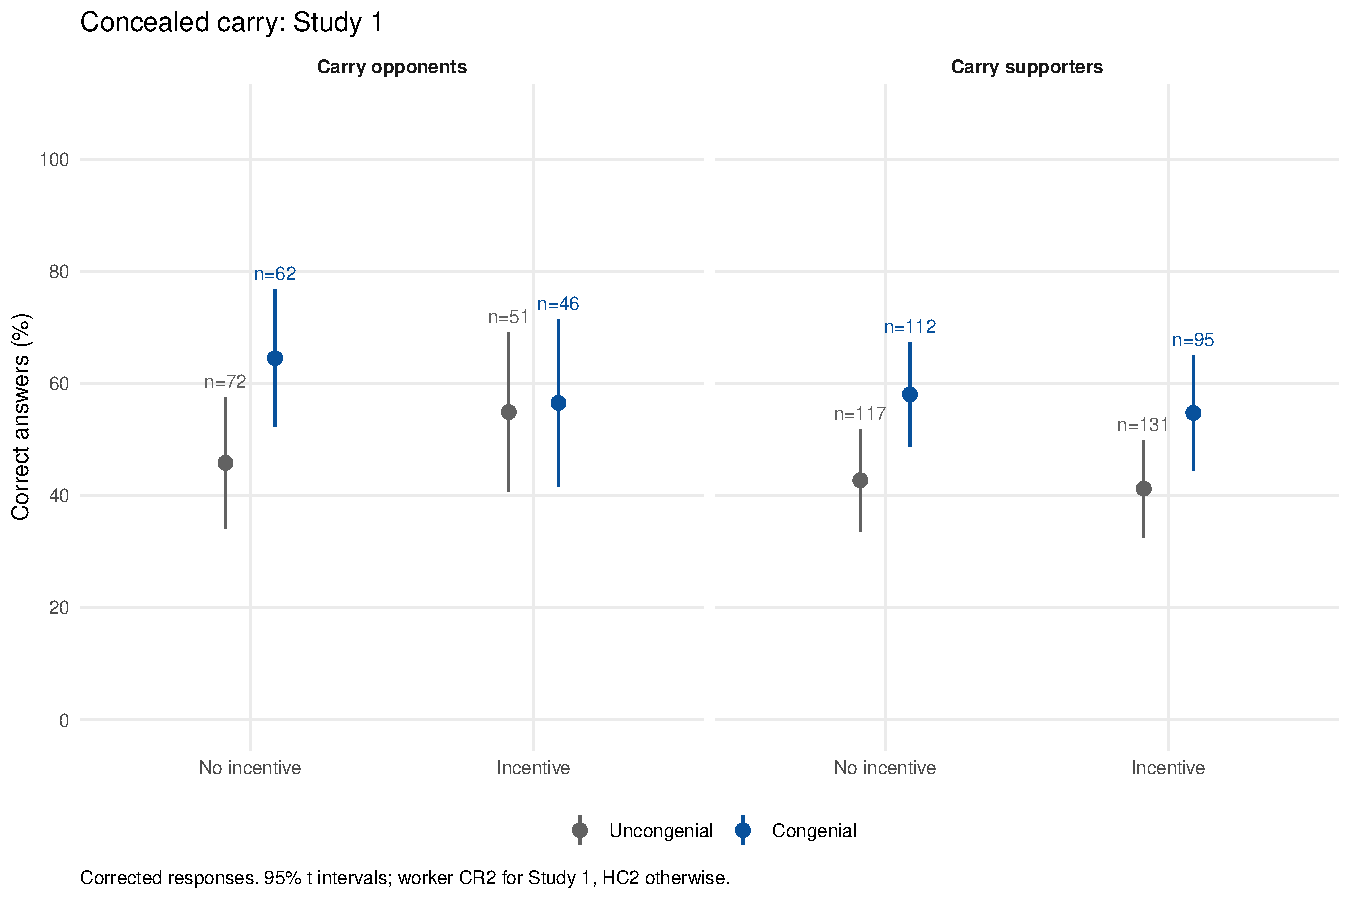
\includegraphics[width=.95\linewidth,height=.34\textheight,keepaspectratio]{../figs/figure_si_5.pdf}
\par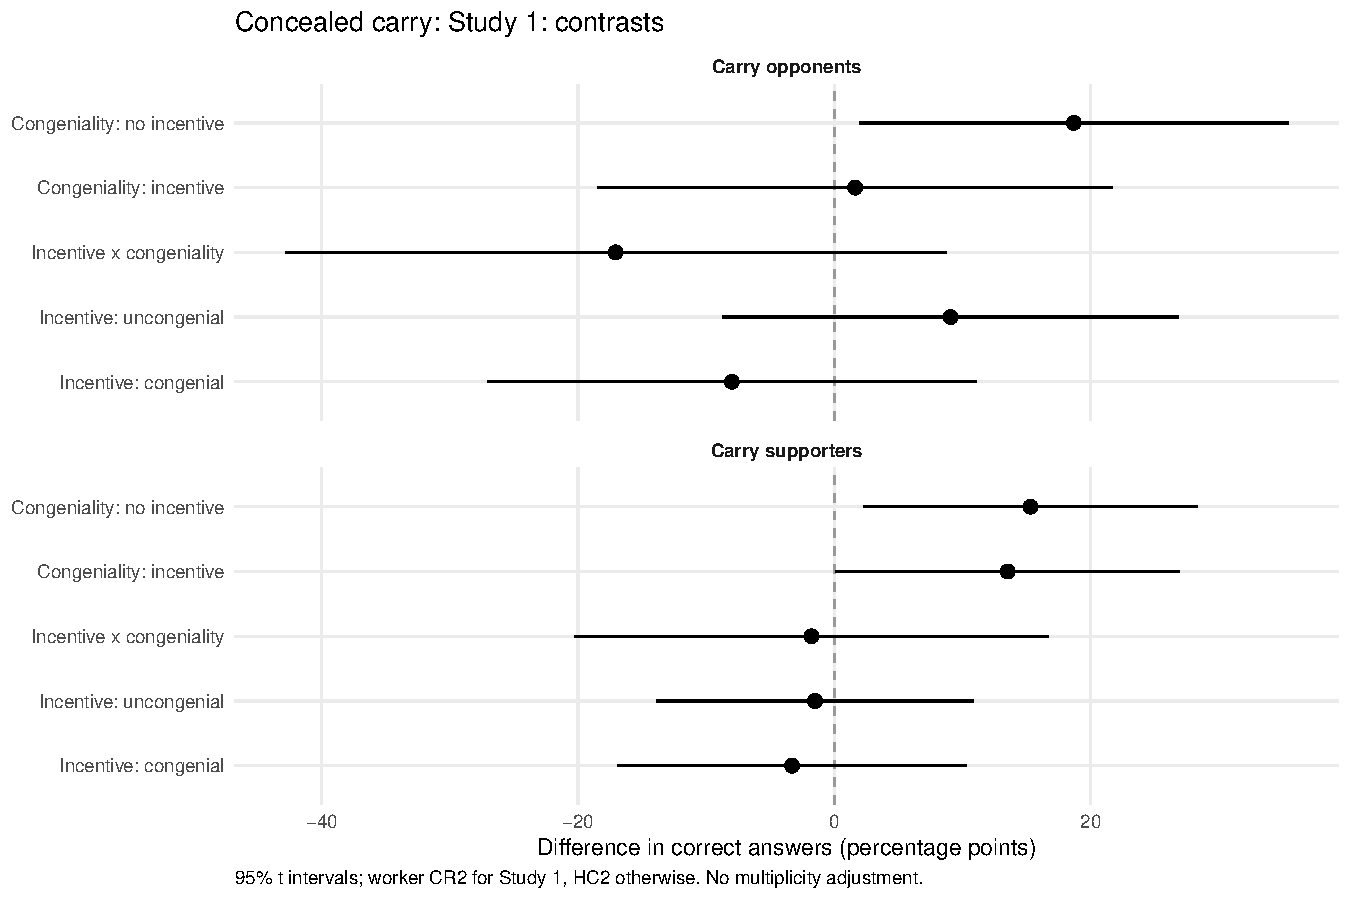
\includegraphics[width=.95\linewidth,height=.34\textheight,keepaspectratio]{../figs/figure_si_5_contrasts.pdf}
\caption{Concealed carry, Study 1. Upper: correctness by condition. Lower: treatment contrasts. Groups are named in each panel. Intervals are 95\% t intervals, with worker-cluster CR2 for Study 1 samples and HC2 otherwise.}\label{fig:study1}
\end{figure}

\begin{figure}[p]
\centering
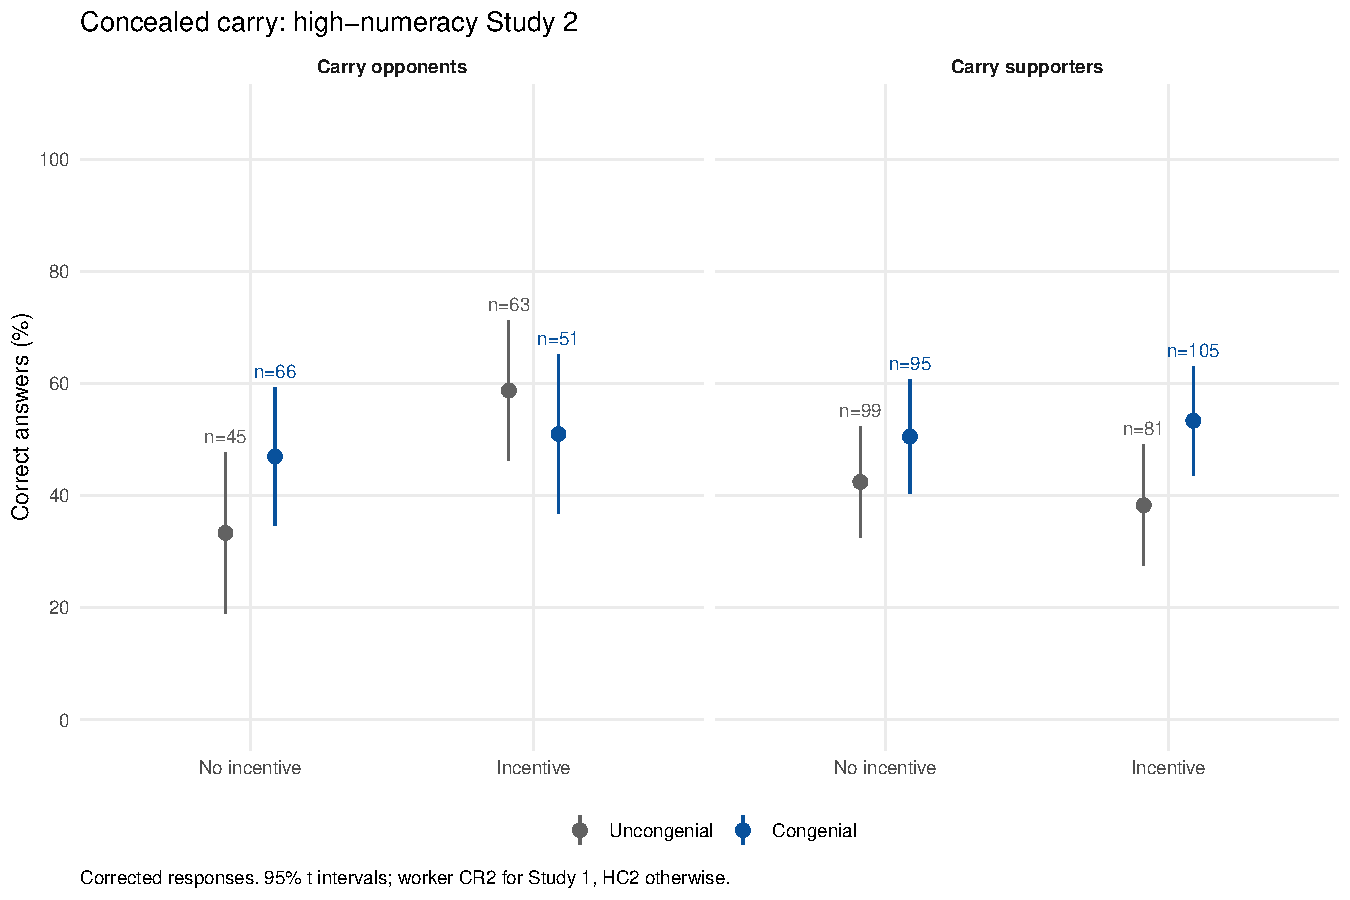
\includegraphics[width=.95\linewidth,height=.34\textheight,keepaspectratio]{../figs/figure_si_6.pdf}
\par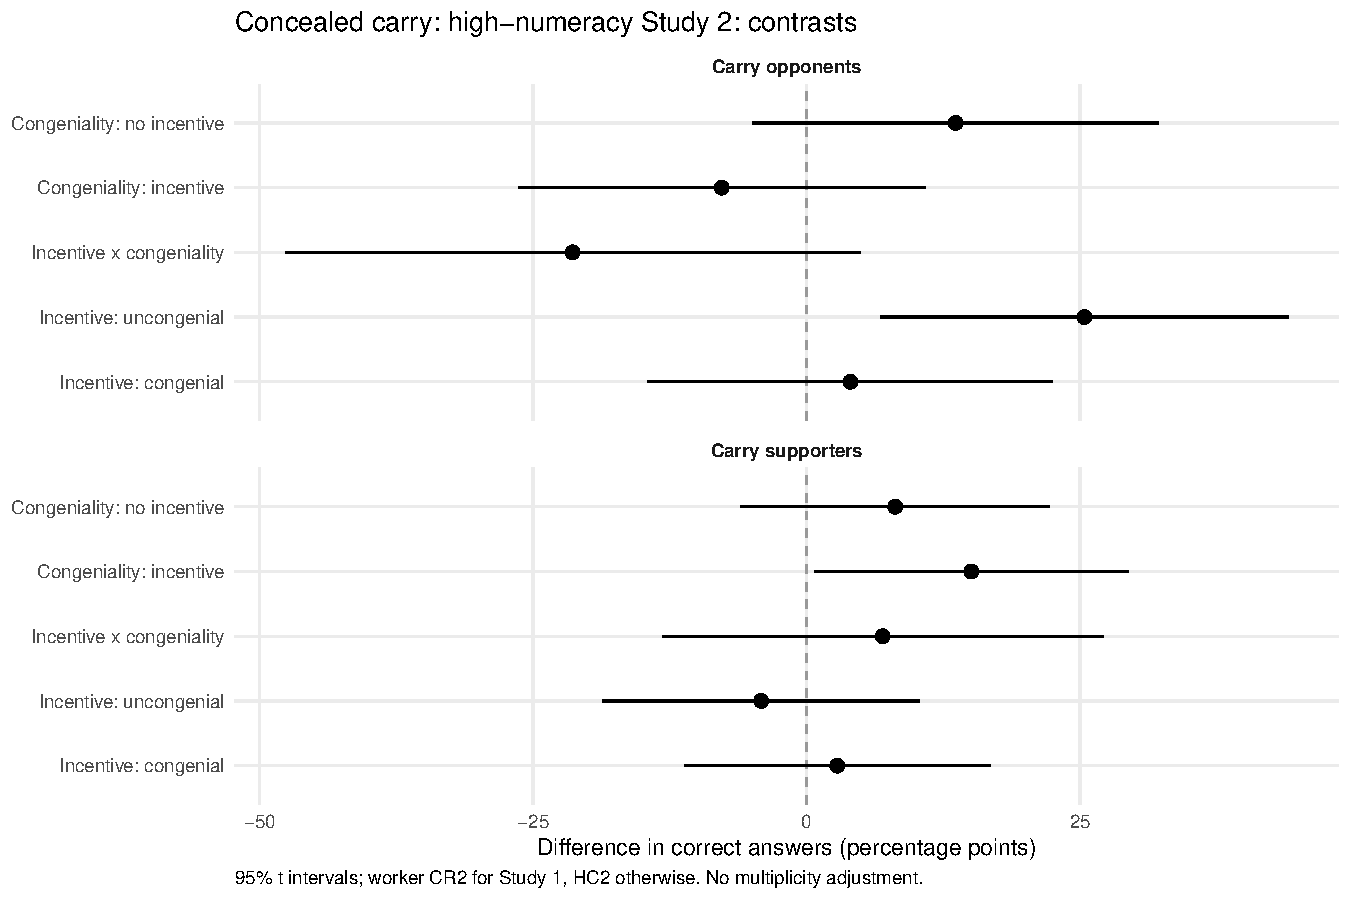
\includegraphics[width=.95\linewidth,height=.34\textheight,keepaspectratio]{../figs/figure_si_6_contrasts.pdf}
\caption{Concealed carry, high-numeracy Study 2. Upper: correctness by condition. Lower: treatment contrasts. Groups are named in each panel. Intervals are 95\% t intervals, with worker-cluster CR2 for Study 1 samples and HC2 otherwise.}\label{fig:study2}
\end{figure}

Figures~\ref{fig:study2_wage} and~\ref{fig:study3_wage} show the minimum wage results separately. Study 2's figure includes wage supporters; Study 3's includes both policy groups. Among Study 3 wage opponents, the interaction is \result{accuracy.figure_si_8.wage_opponents.interaction.estimate.one} points (95\% CI \result{accuracy.figure_si_8.wage_opponents.interaction.ci}; $p\result{accuracy.figure_si_8.wage_opponents.interaction.p}$), so the estimated attenuation remains uncertain.

\begin{figure}[p]
\centering
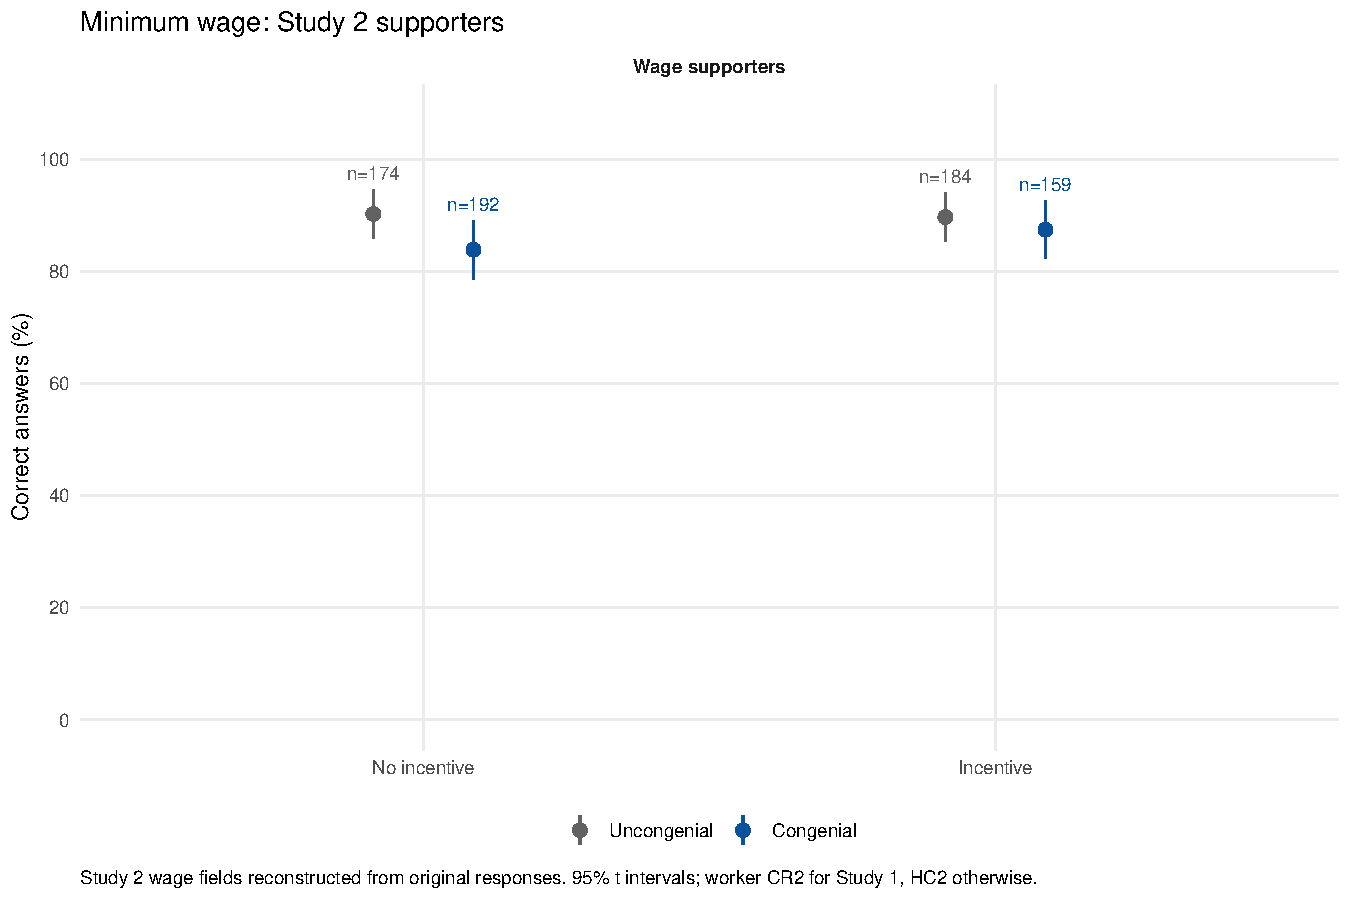
\includegraphics[width=.95\linewidth,height=.34\textheight,keepaspectratio]{../figs/figure_si_7.pdf}
\par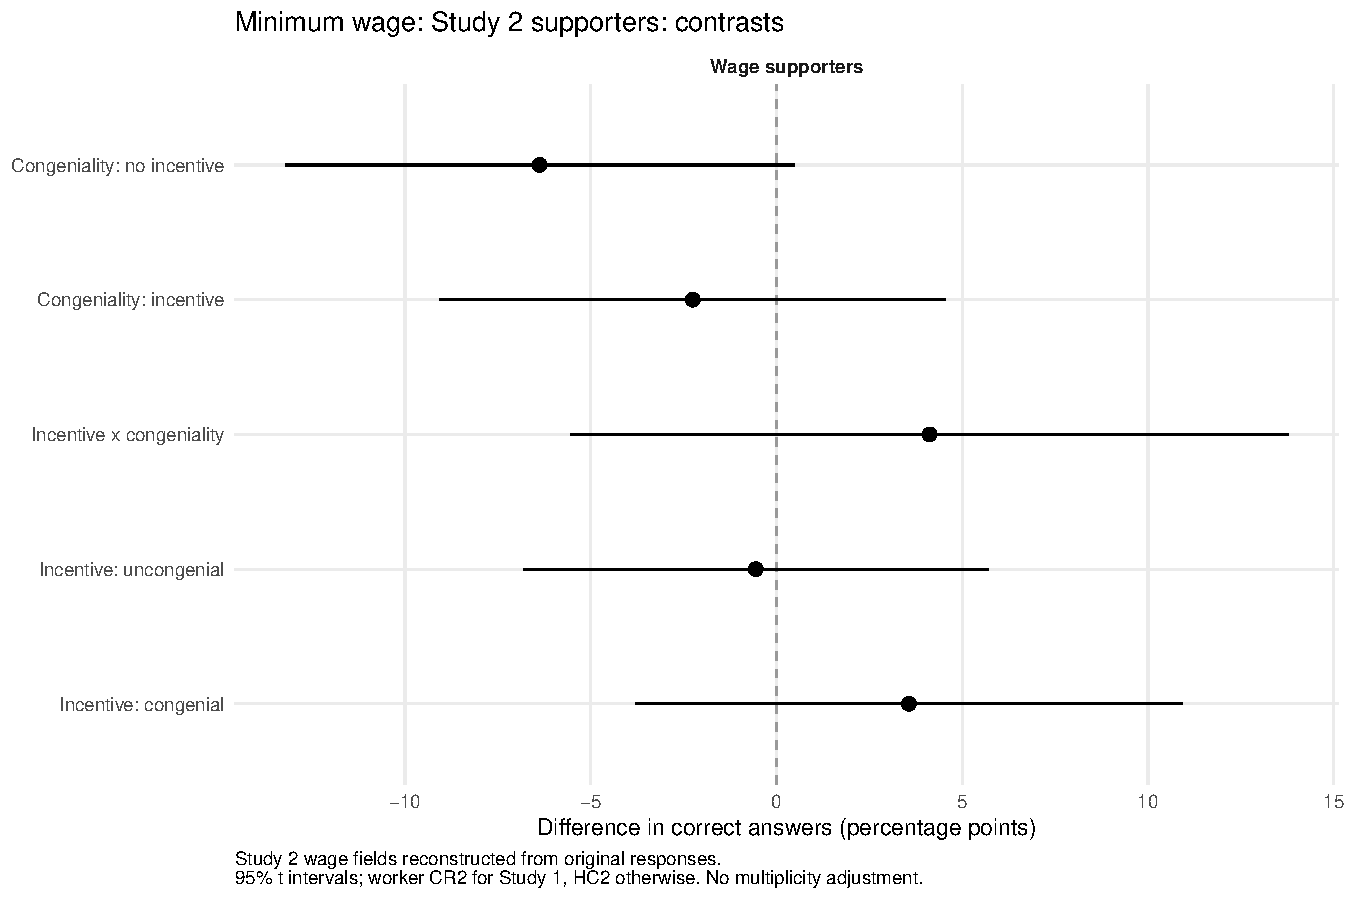
\includegraphics[width=.95\linewidth,height=.34\textheight,keepaspectratio]{../figs/figure_si_7_contrasts.pdf}
\caption{Minimum wage, Study 2 supporters. Upper: correctness by condition. Lower: treatment contrasts. Groups are named in each panel. Intervals are 95\% t intervals, with worker-cluster CR2 for Study 1 samples and HC2 otherwise.}\label{fig:study2_wage}
\end{figure}

\begin{figure}[p]
\centering
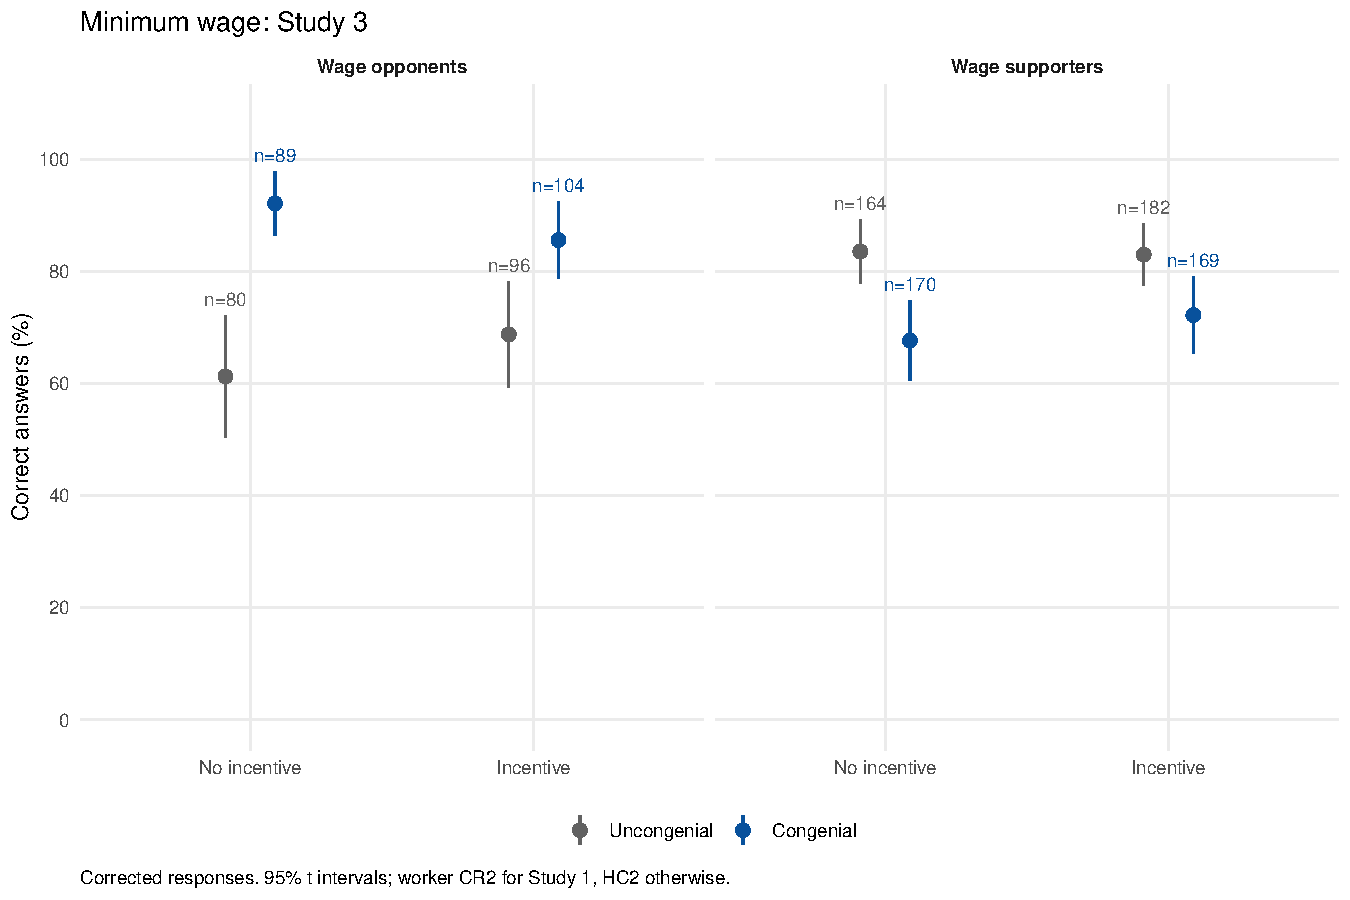
\includegraphics[width=.95\linewidth,height=.34\textheight,keepaspectratio]{../figs/figure_si_8.pdf}
\par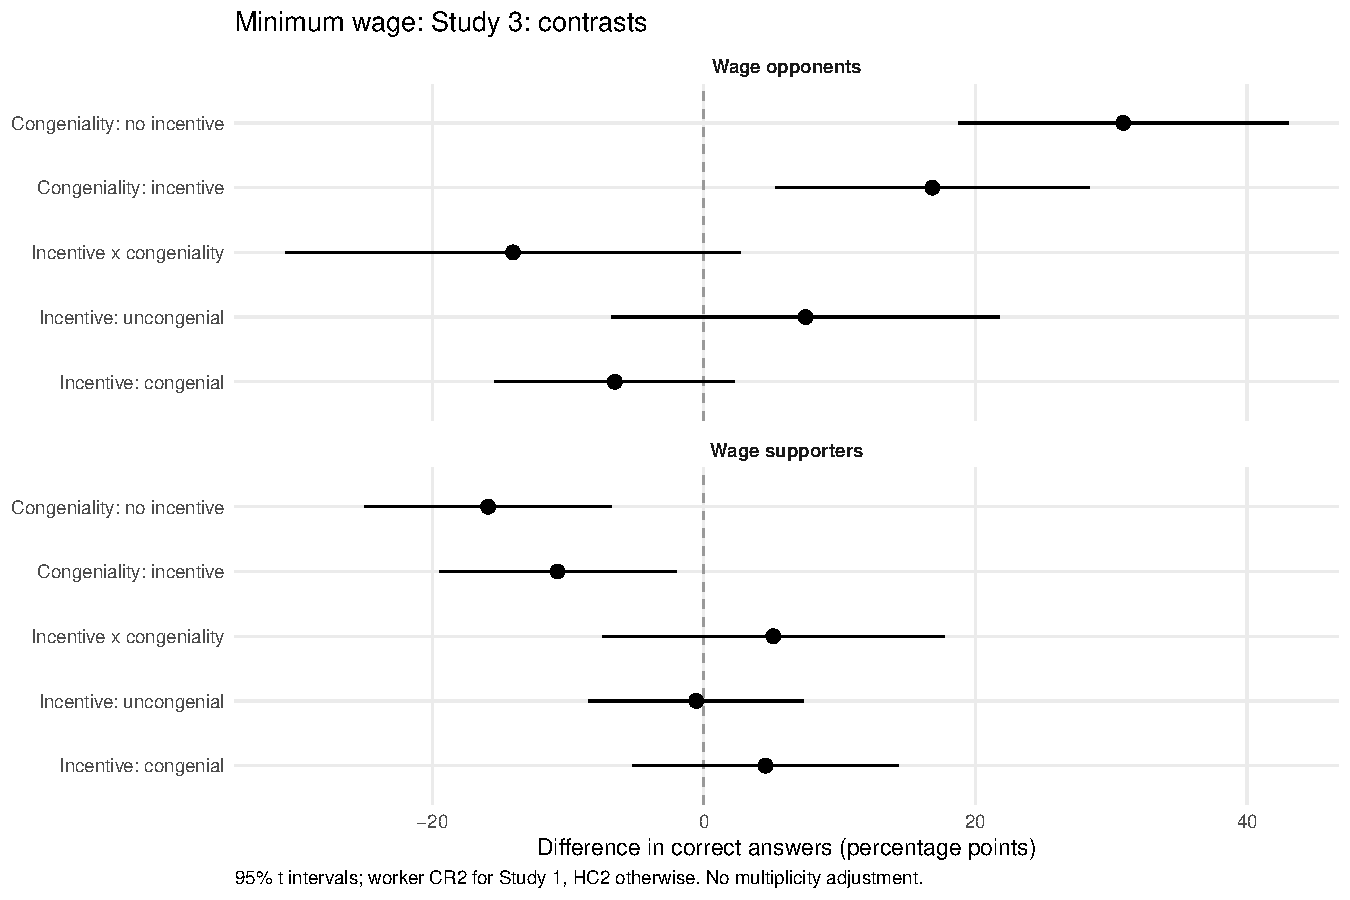
\includegraphics[width=.95\linewidth,height=.34\textheight,keepaspectratio]{../figs/figure_si_8_contrasts.pdf}
\caption{Minimum wage, Study 3. Upper: correctness by condition. Lower: treatment contrasts. Groups are named in each panel. Intervals are 95\% t intervals, with worker-cluster CR2 for Study 1 samples and HC2 otherwise.}\label{fig:study3_wage}
\end{figure}


\clearpage
\subsection{Concealed Carry Task Results as Logistic Regressions}
\label{sec:logit}
\doublespacing

Tables~\ref{tab:logit1} and~\ref{tab:logit2} report logistic specifications for concealed carry supporters and opponents, pooling Study 1 and high-numeracy Study 2. Coefficients are log odds; odds ratios and complete-case N are also shown. These tables retain classical model-based inference for comparison; primary probability contrasts use worker-cluster CR2. The opponent interaction is negative, but the classical two-sided test does not establish a reduction at the .05 level ($p\result{model.gun_logit_position_1.classical.gun_congenial_gun_incentive.p}$).

\bigskip
\begingroup\footnotesize\singlespacing

\begin{longtable}[t]{lllrrlrr}
\caption{\label{tab:logit1}Gun correctness: carry supporters}\\
\toprule
Model & Term & Covariance & Estimate & SE & p & N & OR\\
\midrule
\endfirsthead
\toprule
Model & Term & Covariance & Estimate & SE & p & N & OR\\
\midrule
\endhead
Gun 0 & Intercept & classical & -0.298 & 0.138 & 0.030 & 835 & 0.742\\
Gun 0 & GC & classical & 0.483 & 0.196 & 0.014 & 835 & 1.620\\
Gun 0 & GI & classical & -0.103 & 0.196 & 0.600 & 835 & 0.902\\
Gun 0 & GC:GI & classical & 0.079 & 0.280 & 0.777 & 835 & 1.083\\
\bottomrule
\end{longtable}
\noindent\footnotesize GC/GI: gun congeniality/incentive. Model: ban support (1=yes). Coefficients: log odds; OR: odds ratio. Colons denote interactions. N is the fitted complete-case sample.\par\normalsize

\endgroup
\normalsize
\doublespacing

\begingroup\footnotesize\singlespacing

\begin{longtable}[t]{lllrrlrr}
\caption{\label{tab:logit2}Gun correctness: carry opponents}\\
\toprule
Model & Term & Covariance & Estimate & SE & p & N & OR\\
\midrule
\endfirsthead
\toprule
Model & Term & Covariance & Estimate & SE & p & N & OR\\
\midrule
\endhead
Gun 1 & Intercept & classical & -0.363 & 0.188 & 0.054 & 456 & 0.696\\
Gun 1 & GC & classical & 0.583 & 0.259 & 0.024 & 456 & 1.791\\
Gun 1 & GI & classical & 0.645 & 0.267 & 0.016 & 456 & 1.907\\
Gun 1 & GC:GI & classical & -0.721 & 0.380 & 0.058 & 456 & 0.486\\
\bottomrule
\end{longtable}
\noindent\footnotesize GC/GI: gun congeniality/incentive. Model: ban support (1=yes). Coefficients: log odds; OR: odds ratio. Colons denote interactions. N is the fitted complete-case sample.\par\normalsize

\endgroup
\normalsize
\doublespacing


\clearpage
\subsection{Assessing Experimenter Demand Effects}
\label{sec:demand}

To earn a little extra money, do respondents report what they think the experimenter believes is true instead of what they believe to be true? To answer that, we need to conjecture about respondents' beliefs about the experimenter conducting the study. We consider two hypotheses about what respondents may think in this regard. The first is that respondents believe that most social scientists are liberal, and therefore infer that the result favoring gun control will always be treated as correct. Another is that respondents interpret financial incentives as a cue that the uncongenial option is the right one. We investigate both possibilities.

If respondents believe the experimenter is liberal, incentives should encourage selection of the anti-gun answer regardless of the data. Table~\ref{tab:demand_opp} reports observed answer directions among concealed carry opponents. In the uncongenial condition, incentives reduce the share choosing the congenial anti-gun answer. This pattern conflicts with that simple prediction. Unanswered items are excluded from these response-direction tables rather than assigned an inferred answer.

Among concealed carry supporters, the observed shares choosing the congenial answer are similar across incentive conditions (Table~\ref{tab:demand_supp}). These descriptive comparisons do not establish that incentives have exactly zero effect.

\singlespacing
\begingroup\footnotesize\singlespacing

\begin{longtable}[t]{lrrrrr}
\caption{\label{tab:demand_opp}Reported answer direction: carry opponents}\\
\toprule
Sample & Incentive & Congenial & Congenial answer (\%) & Odds & N\\
\midrule
\endfirsthead
\toprule
Sample & Incentive & Congenial & Congenial answer (\%) & Odds & N\\
\midrule
\endhead
pooled 1 2 & 0 & 0 & 59.0 & 1.44 & 117\\
pooled 1 2 & 0 & 1 & 55.9 & 1.27 & 127\\
pooled 1 2 & 1 & 0 & 43.0 & 0.75 & 114\\
pooled 1 2 & 1 & 1 & 53.6 & 1.16 & 97\\
\bottomrule
\end{longtable}
\noindent\footnotesize Shares are within the specified treatment cell. Odds are congenial answers divided by uncongenial answers.\par\normalsize

\endgroup
\doublespacing

\singlespacing
\begingroup\footnotesize\singlespacing

\begin{longtable}[t]{lrrrrr}
\caption{\label{tab:demand_supp}Reported answer direction: carry supporters}\\
\toprule
Sample & Incentive & Congenial & Congenial answer (\%) & Odds & N\\
\midrule
\endfirsthead
\toprule
Sample & Incentive & Congenial & Congenial answer (\%) & Odds & N\\
\midrule
\endhead
pooled 1 2 & 0 & 0 & 57.2 & 1.34 & 215\\
pooled 1 2 & 0 & 1 & 54.6 & 1.20 & 207\\
pooled 1 2 & 1 & 0 & 59.9 & 1.49 & 212\\
pooled 1 2 & 1 & 1 & 54.0 & 1.17 & 200\\
\bottomrule
\end{longtable}
\noindent\footnotesize Shares are within the specified treatment cell. Odds are congenial answers divided by uncongenial answers.\par\normalsize

\endgroup
\doublespacing

Do respondents interpret the incentive as a cue that the uncongenial answer is correct regardless of the data? The patterns in Tables~\ref{tab:demand_opp} and~\ref{tab:demand_supp} are not consistent with a universal switch to that answer. These comparisons address two specific demand predictions; they do not rule out all demand effects or uniquely identify truthful reporting.

\clearpage
\subsection{How Confident are Respondents in Their Answers?}
\label{sec:confidence}

In Study 3, respondents rated their confidence after selecting an answer. Table~\ref{tab:confidence} reports joint correctness/confidence percentages among no-incentive respondents with both measures observed. In the concealed carry task, \result{confidence.gun.certain}\% are certain and \result{confidence.gun.incorrect}\% are both certain and incorrect. In the minimum wage task, these shares are \result{confidence.wage.certain}\% and \result{confidence.wage.incorrect}\%. These are joint shares of the observed sample, not error rates conditional on certainty.

\singlespacing
\begingroup\footnotesize\singlespacing

\begin{longtable}[t]{lrrrrr}
\caption{\label{tab:confidence}Confidence and correctness without incentives}\\
\toprule
Task & Confidence & Correct & Count & Joint share (\%) & Denominator\\
\midrule
\endfirsthead
\toprule
Task & Confidence & Correct & Count & Joint share (\%) & Denominator\\
\midrule
\endhead
gun & 1 & 0 & 10 & 1.9 & 525\\
gun & 1 & 1 & 4 & 0.8 & 525\\
gun & 2 & 0 & 41 & 7.8 & 525\\
gun & 2 & 1 & 28 & 5.3 & 525\\
gun & 3 & 0 & 141 & 26.9 & 525\\
gun & 3 & 1 & 67 & 12.8 & 525\\
gun & 4 & 0 & 118 & 22.5 & 525\\
gun & 4 & 1 & 47 & 9.0 & 525\\
gun & 5 & 0 & 55 & 10.5 & 525\\
gun & 5 & 1 & 14 & 2.7 & 525\\
wage & 1 & 0 & 5 & 1.0 & 502\\
wage & 1 & 1 & 6 & 1.2 & 502\\
wage & 2 & 0 & 10 & 2.0 & 502\\
wage & 2 & 1 & 29 & 5.8 & 502\\
wage & 3 & 0 & 57 & 11.4 & 502\\
wage & 3 & 1 & 118 & 23.5 & 502\\
wage & 4 & 0 & 29 & 5.8 & 502\\
wage & 4 & 1 & 131 & 26.1 & 502\\
wage & 5 & 0 & 19 & 3.8 & 502\\
wage & 5 & 1 & 98 & 19.5 & 502\\
\bottomrule
\end{longtable}
\noindent\footnotesize Study 3. Confidence ranges from 1 (not confident at all) to 5 (certain). Joint shares sum to 100\% within task.\par\normalsize

\endgroup

\clearpage
\subsection{Excluding Repeated Worker IDs}
\label{sec:worker_exclusion}

\begingroup\footnotesize\singlespacing

\begin{longtable}[t]{lllrllr}
\caption{\label{tab:worker_exclusion}Excluding all records from repeated Study 1 workers}\\
\toprule
Outcome & Group & Sample & Effect & 95\% interval & p & N\\
\midrule
\endfirsthead
\toprule
Outcome & Group & Sample & Effect & 95\% interval & p & N\\
\midrule
\endhead
Correctness (pp) & Carry opponents & Full & -17.85 & {}[-36.12, 0.41] & 0.055 & 456\\
Correctness (pp) & Carry opponents & Exclude repeats & -20.31 & {}[-39.12, -1.49] & 0.034 & 437\\
Correctness (pp) & Carry supporters & Full & 1.91 & {}[-11.62, 15.44] & 0.782 & 835\\
Correctness (pp) & Carry supporters & Exclude repeats & 1.95 & {}[-11.88, 15.78] & 0.782 & 796\\
Ratings (0--10) & Carry opponents & Full & 0.41 & {}[-0.42, 1.23] & 0.336 & 453\\
Ratings (0--10) & Carry opponents & Exclude repeats & 0.35 & {}[-0.51, 1.21] & 0.422 & 435\\
Ratings (0--10) & Carry supporters & Full & 0.31 & {}[-0.33, 0.95] & 0.344 & 830\\
Ratings (0--10) & Carry supporters & Exclude repeats & 0.31 & {}[-0.34, 0.96] & 0.350 & 793\\
Ratings (0--10) & Pooled & Full & 0.34 & {}[-0.16, 0.85] & 0.180 & 1283\\
Ratings (0--10) & Pooled & Exclude repeats & 0.32 & {}[-0.19, 0.84] & 0.219 & 1228\\
\bottomrule
\end{longtable}
\noindent\footnotesize Incentive-by-congeniality interactions. Study 1 and high-numeracy Study 2; corrected coding. Exclusion removes all 70 records from the 34 IDs repeated within the 785-record Study 1 released sample. Study 2 is unchanged and its records are assumed to be distinct workers. Both samples use CR2 t inference, isolating the sample change. Raw records are preserved.\par\normalsize

\endgroup

\begin{figure}[p]
\centering
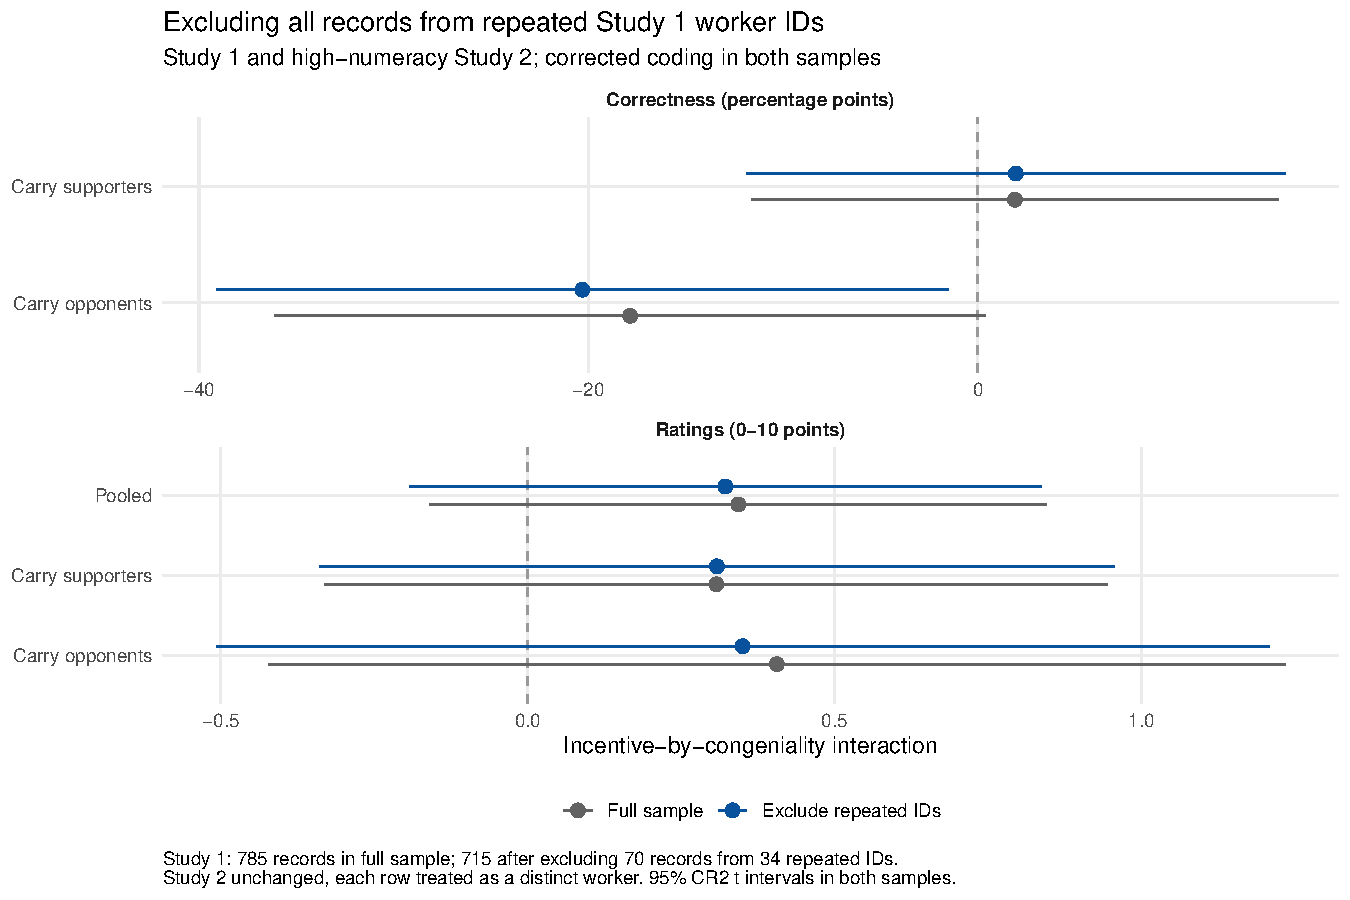
\includegraphics[width=\linewidth]{../figs/worker_exclusion.pdf}
\caption{Incentive-by-congeniality interactions with and without all records from repeated Study 1 worker IDs. Study 2 is restricted to high numeracy and each row is assumed to represent a distinct worker. Both samples use corrected coding and 95\% CR2 t intervals.}\label{fig:worker_exclusion}
\end{figure}
\clearpage

\end{document}
